\chapter{Cells in the Brain}	
\label{chap:cells-CNS}

Neurons, neuroglia (astrocytes and oligodendrocytes), and ependymal cells are
three distinct categories of neural cells in the central nervous system.
\citep{morest2003}.

%There are different cell types in the brain:
\begin{itemize}
  \item glial cells (neuroglia): not conducting electricle signals
  - Sect.\ref{sec:glial-cells}
  
 
  \item nerve cells: can conduct electricle signals - Sect.\ref{sec:nerve-cells}
\end{itemize}

% The CNS is made up of many cells (mainly {\it nerve cells} (or neurons) and {\it
% glial 
% cells})\footnote{\url{http://library.thinkquest.org/2935/Natures_Best/Nat_Best_Low_Level/Nervous_page.L.html}}.

\section{Neuron genesis}
\label{sec:neurogenesis}

Although the vast majority of neurons in the mammalian brain are formed only a
few years after birth, parts of the adult brain retain the ability to grow new
neurons from neural stem cells in a process known as neurogenesis. Neurotrophins
called BDNF (Sect.\ref{sec:BDNF}) help to stimulate and control neurogenesis.

\begin{itemize}
  \item  During development:  One dendrite sprouted an impressive 90 microns
  (about .003 inches), more than doubling its length in less than two weeks.

Shortly after birth in humans, a substantial number of new nerve cells are
produced and added to brain regions called the cerebellum, olfactory bulb,
prefrontal cortex, and hippocampus. 
  
  \item At age of 2: the brain is 80\% the size of an adult brain

Growth rate: 250,000 neurons per minute and then spend the next few years wiring
them together.

After the age of 2, neurogenesis in most of these regions disappears except in
the hippocampus - a region involved in learning and memory. This may be the only
location in the brain where new cells are added throughout one's lifetime.
  
  \item 20-30\% of neurons in neocortex are interneurons

These neurons are believed to play an important role in regulating brain
activity by delaying or blocking signals from excitatory neurons. While
pyramidal neurons didn't exhibit any structural changes, about 14 percent of the
interneurons they observed showed structural modifications.

  \item 
\end{itemize}

\subsection{non-mammal}

Other animals, such as fish, amphibians, reptiles, and birds display a
continuous addition and high turnover of nerve cells in many brain structures
throughout life.

\subsection{mammals}

In adult mammals, the birth of new neurons becomes more limited.
In rodents, only two regions of the brain continue to acquire new nerve cells
throughout life; however, in adult humans the only remnant of neurogenesis
persists in one part of the hippocampus.


% Bergmann O, Liebl J, Bernard S, Alkass K, Yeung MSY, et al. The age of olfactory bulb neurons in humans. Neuron. 74, 634-639 (2012).
% 
% BhardwajRD, Curtis MA, Spalding KL, Buchholz BA, Fink D, et al. Neocortical neurogenesis in humans is restricted to development. Proc. Nat Acad. Sci. 103, 12564-12548 (2006).
% 
% Eriksson PS, Perfilieva E, Bjork-Eriksson T, Alborn A, Nordborg C, et al. Neurogenesis in the adult human hippocampus. Nature Medicine. 4, 1313-1317 (1998).
% 
% Rakic P. Neurogenesis in adult primate neocortex: an evaluation of the evidence. Nature Reviews Neuroscience. 3, 65-71 (2002).
% 
% Knoth R, Singec I, Ditter M, Pantazis G, Capetian P.  Murine features of neurogenesis in the human hippocampus across the lifespan from 0 to 100 years. PLoS ONE. 5, e8809 (2010).

Within the brain of adult mammals, proliferation of neurons occurs spontaneously
in the walls of the lateral ventricle and the subgranular layer of the
hippocampus.
\begin{enumerate}
  \item Cells from the ventricle walls migrate and integrate into the olfactory
  bulb
  
  \item New neurons in the subgranular layer differentiate into dentate gyrus
  granule cells of the hippocampus 
\end{enumerate}

The functional significance of adult-born neurons in the hippocampus is still
debated, with opposite results in  hippocampus-dependent learning and memory
tasks.  This raises the question of how important adult neurogenesis might be
for animals living in their natural context, and to what extent experimentally
obtained insights into the regulation and function of adult hippocampal
neurogenesis (AHN) can help us to understand its relevance in the healthy and
diseased human brain.

AHN is most prominent in rodents, but shows considerable variability across
species, being lowest or missing in primates and bats.
However, as only a fraction of mammalian species has been investigated, further
comparative studies are necessary in order to recognize whether AHN has a common
unique function, or whether it mediates species-specific hippocampal functions
\citep{amrein2009}


\section{Progenitor cells}
\label{sec:progenitor-cell}


One of the most challenging areas in neuroscience is understanding the genetic
and extrinsic mechanisms that direct cell fate decisions. 

The telencephalon (Sect.\ref{sec:telencephalon}) contains two main classes of
neural progenitors. {\bf Apical progenitors} (APs) divide along the ventricular
surface, whereas {\bf basal progenitors} (BPs) divide within the subventricular
zone (SVZ).

In the developing cerebral cortex, the BP population expands as neurogenesis
proceeds, BP-derived neurons populate all cortical levels, and disrupting BP
generation alters cortical size and lamination.

Similar types of APs, BPs and modes of neurogenesis are observed in the
subpallium, the source of all telencephalic GABAergic interneurons
(Sect.\ref{sec:GABAergic-neurons}).


Petros et al. (2015) showed that apical versus basal neurogenesis influences the
fate determination of major subgroups of cortical interneurons derived from the
subcortical telencephalon.
\begin{itemize}
  \item  Somatostatin-expressing interneurons arise mainly from apical divisions
  along the ventricular surface, whereas 
  \item parvalbumin-expressing interneurons
  originate predominantly from basal divisions in the subventricular zone 
\end{itemize}


\section{Glial Cells (neuroglia) Types}
\label{sec:glial-cells}

Glial cells (neuroglia) \footnote{aka supporting cells} (glia in Greek for
``glue'') refers to a group of non-neuronal cells that provide the nerve cells
physical supports, nutrition, and {\it participates in signal transmission} in
the nervous system. In human brain, glial cells outnumber neurons by about 10 to
1. Glial cells can be found in both CNS and PNS.


For centuries, it is believed that glial cells play no roles in
neurotransmission, but only to provide physical support for neurons. This has
been changed (see at the end of the section).
\textcolor{red}{The only notable differences between neurons and glial cells are
neurons' possession of axons and dendrites, and capacity to generate action
potentials.}

There are several types of glial cells:
\begin{itemize}
  \item In CNS:
\begin{enumerate}
  
  \item {\bf astrocytes} (astroglia): a star-shaped glial cell
  (Sect.\ref{sec:astrocytes})
    
  \item {\bf microglial cells}: extremely small cells -
  Sect.\ref{sec:microglial-cell}
  
  \item {\bf oligodendrocytes} (oligodendroglia, Greek = cells with a few
  branches): wrap around the nerve cells and form the myelinated sheaths
  (Sect.\ref{sec:oligodendrocytes})
  
  \item {\bf NG2 cells} - Sect.\ref{sec:NG2-cell}
  
%  \item {\bf Schwann cells} - Sect.\ref{sec:Schwann_cells}
  
  \item {\bf Bergmann cells} - Sect.\ref{sec:Bergmann-cells}
  
  \item {\bf Muller cells} - Sect.\ref{sec:Muller-cells}
  
  \item {\bf ependymal cells}: Sect.\ref{sec:ependymal-cell}
  
\end{enumerate}

  \item In PNS: 
\begin{enumerate}
    \item {\bf Schwann cells} (neurolemmocytes): wrap around the nerve cells
    and form the myelinated sheaths to facilitate the impulse conduction
    (Sect.\ref{sec:Schwann_cells}).

   \item {\bf satellite cells}: provide structural support and
regulate the exchange of materials between
neuronal cell bodies and interstitial fluid    
\end{enumerate}
\end{itemize}
Glial cells could interfere with synaptic transmission by communicating with
neurons via the extracellular space, e.g., by modulating ion concentrations or
transmitter levels in the cleft.

Both Oligodendrocytes and Schwann cells indirectly assist in the conduction of
impulses by forming myelin sheath (which  is 80\% lipid and 20\% protein) to
facilitate the impulse conduction.
As a result, myelinated nerves can conduct impulses quicker than unmyelinated
ones. A single oligodendrocyte can extend its processes upto 50-60 axons,
wrapping approximately 1 $\mum$ of myelin sheath around each axon.
Schwann cells, on the other hand, can wrap around only 1 axon The part of the
axon with diameter of just about 1$\mu m$, wrapped by Schwann cells which can be
in the order of a few millimetres.

In 21st century, there are evidences that glial cells do have some effects on
certain physiological processes, e.g. breathing and in support nerve cells to
form synaptic connections (Sect.\ref{sec:synapse}). Those in the hippocampus
(Sect.\ref{sec:hippocampus}) and cerebellum (Sect.\ref{sec:cerebellum}) also
participate in neurotransmission.

\subsection{Astrocytes (in CNS)}
\label{sec:astrocytes}

Astrocytes are star-shaped cells whose presence varies from region to region in
the brain and spinal cord. Depending on staining techniques, glial cells are
estimated from 20-40\% of all glia cells. Modeling astrocytes is discussed in
Chap.\ref{sec:astrocyte-modeling}.

Of 11 distinct phenotypes that can be readily distinguishe, 8 involve specific
interactions with blood capilaries (Sect.\ref{sec:blood-brain-barrier}).
There is strong evidence that astrocytes (Sect.\ref{sec:astrocytes}) can update
regulate many blood-brain barrier, including leading to tighter tight junctions, 
expression and polarized localization of transporters (Pgp, GLUT1), and
specialized enzyme systems (Review: Abbott, Hansson, 2006).

There are major discoveries that bring new understanding to the role of
astrocytes. Astrocytes
\begin{enumerate}
  \item ubiquitous 'glue' that holds the tissue together and keep it working
  properly, e.g. regulate the concentration of ions and neurotransmitters in the
  extracellular space to prevent the products of neural activity from building
  up and interfering with network function, a bit like a housekeeper who vacuums
  and washes the dishes after a part.
  
  
  \item  facilitate intercellular $\Ca$ waves over long distances by releasing
  {\it gliotransmitter} in a $\Ca$-dependent manner.

  \item  Some data also suggest astrocytes release {\it glutamate}
(Sect.\ref{sec:glutamate_receptor}) through $\Ca$-dependent manner.
\url{http://en.wikipedia.org/wiki/Astrocyte}
  
  \item
  suppress the repair process in CNS, i.e. it produces inhibitory molecules that
  inhibit regrowth of a damaged or severed axon.
\end{enumerate}

\subsection{-- perivascular endfeet}
\label{sec:astrocyte-perivascular-endfeet}

The perivascular endfeet of astrocytes, which are closely applied to the
microvessel wall, show several specialized features characteristic of this
location
\begin{enumerate}
  \item high density of orthogonal arrays of particles (OAPs): containing water
  channel aquaporin 4 (AQP4); Kir4.1 K+ channel (Sect.\ref{sec:Kir4.1})
  
  They involve in volume regulation and ion regulation.
  
  \item 
\end{enumerate}


\subsection{Microglial cells}
\label{sec:microglial-cell}
  
{\bf Microglial cells} are highly mobile and are the primary immune cells of the
CNS which function as phagocytes, i.e. cells in the body that remove cellular
waste, damaged nervous tissue and protect against microorganism.
% Microglial cells have important roles in maintaining brain homeostasis, and
% they are implicated in multiple brain diseases.
% Microglia  are the primary immune cells of the CNS, and are highly similar to
% peripheral macrophages.

They respond to pathogens and injury by becoming "activated"
- a process whereby they rapidly change morphology, proliferate and migrate to
the site of infection/injury where they phagocytose and destroy pathogens as
well as remove damaged cells.
\begin{enumerate}
  \item secrete cytokines and chemokines, as well as prostaglandins, NO and
  reactive oxygen species, which help to elevate and direct the immune response. 
  
  \item instrumental in the resolution of the inflammatory response, through the
  production of anti-inflammatory cytokines such as Il-10.
\end{enumerate}


{\bf IMPORTANT}: Microglial cells (in adult brain) are fully dependent upon 
Colony-Stimulating Factor 1 receptor (CSF1R) signaling for their survival
(Sect.\ref{sec:CSF1R})
\begin{enumerate}
  \item  administration of specific CSF1R inhibitors that cross the blood brain
  barrier $\rightarrow$  rapid elimination of microglia from the adult brain
  
NOTE: Using PLX3397 (a dual CSF1R inhibitor and c-kit kinase inhibitor) within 7
days of continuous treatment ~80\% of all microglia are eliminated, and by 21
days of continual treatment >95\% of all microglia are eliminated (Green Lab).
Microglia remain eliminated for as long as we continue CSF1R inhibitor treatment. 
\url{http://faculty.sites.uci.edu/kimgreen/bio/microglia-in-the-healthy-brain/}
 
NOTE: Using  PLX5622 (specific CSF1R inhibitor with KI = 5.9 nM with at least
50-fold selectivity over 4 related kinases, and over 100-fold selectivity
against a panel of 230 kinases) is also enough to help eliminate microglial
(Dagher - Green, 2015).

Dose-dependent of microglial cell elimination: Dagher et al. (2015)

 
\end{enumerate}


\subsection{--- microglial cell migration}



\subsection{--- microglial in brain diseases}

While microglia are crucial for the protection of the CNS from pathogens, as
well as in clearing up cellular debris following cell death or minor injuries,
microglial cells may also play harmful roles in neurodegenerative diseases and
brain injuries. Microglia are negatively implicated in Alzheimer's disease.
Parkinson's disease, Huntington's disease, Frontal Temporal dementias, ALS,
Traumatic Brain Injuries, Ischaemic Strokes, Epilepsy, and many more.
% , such as Alzheimer's disease, Parkinson's disease, ischemic injury, and
% traumatic brain injuries

GENERAL CONCENSUS:
\begin{itemize}
  \item  microglia mount an initial beneficial response, helping to limit damage
  from injury, or  phagocytosing aggregating toxic peptides such as A$\beta$ 
  and perhaps limiting plaque formation.
  
  \item 
\end{itemize}




\subsection{Oligodendrocytes (in CNS)}
\label{sec:oligodendrocytes}

These dendrocytes resemble an octopus bulbous body and contain up to fifteen
arm-like processes. Each ``arm" reaches out to a nerve fiber
(Sect.\ref{sec:Axon}) and spirals around it, creating a myelin sheath,
Fig.\ref{fig:oligodendrocytes}. Each oligodendrocyte forms one segment of myelin
sheath for several adjacent axons.

\begin{figure}[htb]
  \centerline{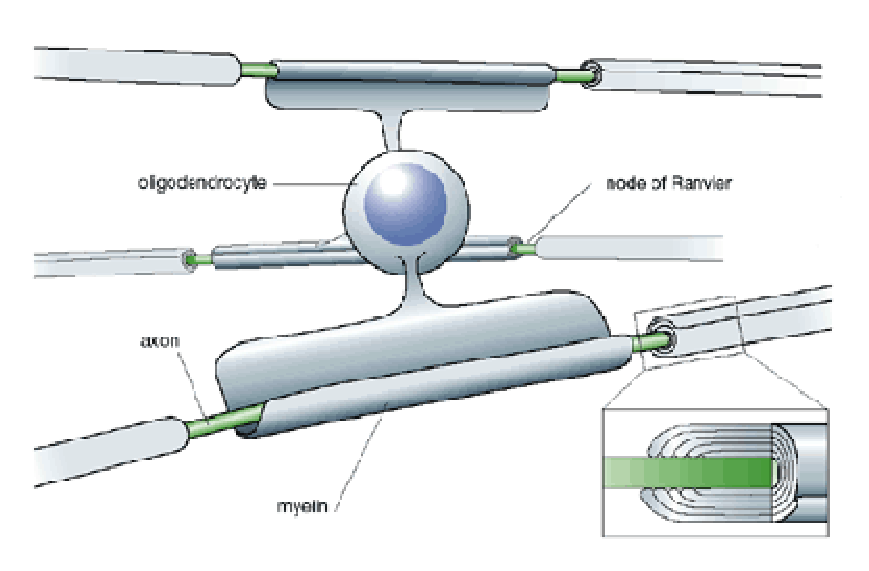
\includegraphics[height=6cm]{./images/oligodendrocyte.eps}}
  \caption{An oligodendrocyte with arms reaching to
  different axons}\label{fig:oligodendrocytes}
%http://www.nature.com/ng/journal/v33/n3/full/ng0303-327.html  
\end{figure}

\subsection{NG2 cell (polydendrocyte)}
\label{sec:NG2-cell}
\label{sec:polydendrocyte}

{\bf NG2 cells} (polydendrocyte) is a population of CNS cells that are distinct
from neurons, mature oligodendrocytes, astrocytes and microglia.
They express proteoglycan NG2

\textcolor{red}{\bf Morphology}:
\begin{enumerate}
  \item highly branched morphology
  
  \item distributed throughout the grey and white matter
  
  \item {\it in vitro}: they can differentiate into oligodendrocyte
  (Sect.\ref{sec:oligodendrocytes}), so they have often been considered as
  precursor cell of oligodendrocyte.
  
  Whether polydendrocytes are multipotential cells that can give rise to neurons
  and astrocytes as well as oligodendrocytes is now highly debated (Nishiyama
  et al., 2009).
  
  \item  electrophysiological studies indicate that polydendrocytes receive
  synaptic input from neurons, suggesting that they are integrated in the neural
  network. 
\end{enumerate}


\subsection{Radial glia cell}
\label{sec:Radial-glial}



\subsection{-- Muller cell}
\label{sec:Muller-cell}

 Muller cells, are a type of vertebrate retinal glial cells (the most common
 type of glial cell in retina and span across the entire thickness of the neural
 retina), first recognized and described by Heinrich Muller.
 
They maintain the stability of the retinal extracellular environment by
regulation of K+ levels, uptake of neurotransmitters (ACh and GABA
specifically), removal of debris, storage of glycogen, electrical insulation of
receptors and other neurons, and mechanical  support of the neural retina.

Muller glia are radial glial cells (Sect.\ref{sec:Radial-glial}) and Muller glia
are currently being studied for their role in neural regeneration, a phenomenon
that is not known to occur in humans. In animal (e.g. zebra fish), Muller cells
can undergo differentiation into multipotent progenitor cells, e.g.
functioning as stem cells.

\subsection{-- Bergmann cells}
\label{sec:Bergmann-cells}


\begin{mdframed}

The cerebellum of all vertebrates contains specialized {\it radial astrocytes},
which send long, vertically oriented processes toward the pia. These glial
processes were discovered by Karl Bergmann in 1857 as {\it cerebellar radial
fibers}.
In 1871, Camillo Golgi recognized these structures as cells and found their
somata/cell bodies, from where the radial fibers originated. Both Golgi and
Ramon-y-Cajal referred to these cells as epithelial cells, and for many years
they were generally known as {\it Golgi epithelial cells}. In recent times, the
common name for these cerebellar radial astrocytes is {\bf Bergmann glial
cells}.
\end{mdframed}

The Bergmann glia is composed of unipolar protoplasmic astrocytes in the
cerebellar cortex. Bergmann glial cells locate their cell bodies around Purkinje
cells, and extend radial or Bergmann fibers enwrapping synapses on Purkinje cell
dendrites.  Bergmann glial cells play an important role in the development of
the cerebellum 

\begin{enumerate}
  \item CLASSIC VIEW:  they were thought to serve as passive insulators of the Purkinje
cell.
  
  \item NOVEL VIEW: Bergmann glial cells are equipped with a large repertoire of
  receptors allowing them to sense the activity of synapses (Muller,
  Kettenmann, 1995).
  
  These receptors have distinct biophysical and pharmacological features
  activating second-messenger pathways in the Bergmann glial cells. 
  
\end{enumerate}


\textcolor{red}{\bf Morphology}: Verkhratsky, Reichenbach (2009)
\begin{enumerate}
  \item 3-6 stem processes, protrude through the molecular layer toward pia
  surface
  
  These processes contain many mitochondria and bundles of intermediate
filaments, constituted by vimentin and glial fibrillary acidic protein (GFAP).

On average, every Bergmann glial cell in rodent cerebellum has a volume of
approximately 3600 $\mum^3$; and together these cells occupy approximately
15-18\% of the volume of the molecular layer.

  \item The stem processes of Bergmann glial cells end at the pia mater, with
  so-called endfeet, which together form a complete covering of the cerebellar
  surface.

On their way from soma to the pia, the stem processes extend numerous side
branches, which form close contacts with synapses present on the dendrites of
Purkinje neurons; on average, every Bergmann glial cell covers 2000-6000 such
synapses.

  \item approximately eight Bergman glial cells per every Purkinje neuron

  \item 
\end{enumerate}

\subsection{Schwann cells (in PNS)}
\label{sec:Schwann_cells}

The outermost nucleated cytoplasmic layer of the Schwann cell that surroudn
the axon of the nerve cell is called {\bf neurolemma} (neurilemma, or
sheath of Schwann).

Schwann cells are also known as neuri-lemmocytes. These cells envelop nerve
fibers of the PNS by winding repeatedly around a nerve fiber with the nucleus
inside of it. This process creates a myelin sheath, which not only aids in
conductivity but also assists in the regeneration of damaged fibers.
Unlike astrocytes in CNS (Sect.\ref{sec:astrocytes}), Schwann cells promote
repair of damaged nerve cells.
This difference between the CNS and the PNS, raises hopes for the regeneration
of nervous tissue in the CNS.

\subsection{Ependymal cells}
\label{sec:ependymal-cell}
  
Ependymal cells  possesses microvilli and cilia, line the ventricles and central
canal produce and assist in the circulation of Cerebral Spinal Fluid.

\section{Neuron type classification}
\label{sec:neuron-type-classification}

The classical categorization of neurons was based mainly on the morphology of
the cell body and its dendrite, as seen after Golgi impregnation
(Sect.\ref{sec:neuron-classify-Golgi-1-2}).
\begin{itemize}
  \item Lorente de No (1944) work:
  \item Sholl (1956) work:
\end{itemize}

Nowadays, seeral other criteria have been proposed for categorizing neurons,
e.g. brain region to which the axon projects, the type of synapses made by
neurons (e.g. inhibitory neurons or excitatory neurons), transmitters released
by neurons (e.g. GABAergic neurons, Dopaminergic neurons), and other criteria
(e.g. the presence of certain enzymes, neuropeptides).

There seem to be 2 approaches: (1) one try to create as any categories as
possible, (2) one try to limit the number of categories as much as possible.


% For neurons, in Sect.\ref{sec:nerve-cells}, we have learnt different components
% in a nerve cell. 
No one has an exact number of how many types of neurons, but if
you count all the types and subtypes in the entire nervous system, it can reach
in the hundreds.
 \textcolor{red}{List of all known neurons} in
\begin{itemize}
  \item  NeuroLex.org: NeuroScience Lexicon
  
\url{http://neurolex.org/wiki/Category:Neuron}

  \item NeuroMorpho.org:
   database of digitally reconstructed neurons that you can browse by species,
  brain region and cell type.
  
  \url{http://neuromorpho.org/neuroMorpho/bycell.jsp}
  
  
\end{itemize} 
\url{http://blogs.scientificamerican.com/brainwaves/know-your-neurons-classifying-the-many-types-of-cells-in-the-neuron-forest/}

Example: pyramidal cells, purkinje cells and motoneurons, as shown in
Fig.\ref{fig:neuron_cell}. 


\subsection{Option 1: Golgi 1, Golgi 2}
\label{sec:neuron-classify-Golgi-1-2}
\label{sec:Golgi-I-neurons}
\label{sec:Golgi-II-neurons}

One way to classify the neuron by Camillo Golgi, from the end of 19th century.
 
Once the fresh brain tissue is placed in a concentrated solution of silver
salts. Only a small fraction of the cells are impregnated; and the precipate
fills up the soma and many of the branches of these cells.


\begin{itemize}
  \item  {\bf Golgi 1} (neurons with axon): to move signal over a long distance 
  
  The basic morphology of Golgi I neuron is spinal motor neurons
  (Sect.\ref{sec:spinal-motor-neurons}).
  
  \item {\bf Golgi 2} (neurons without axon): to move signal locally
\end{itemize}
\footnote{\url{http://en.wikipedia.org/wiki/Neuron}}.

Both belong to the multi-polar neurons
(Sect.\ref{sec:neuron-classify-multi-pseudo-bi-polar}).

\subsection{Option (Lorente de No (1944))}

Using Golgi staining method, Lorente de No in 1933 described more than 60 cell
types. 

In 1944, he classified the neurons based on the distributions of axons in
the cortex.
\begin{enumerate}
  \item neurons with axons that grow downward and usually depart the cortex into
  the white matter
  
  These are pyramidal neurons
  
  \item neurons with axons branch out mainly in the vicinity of the cell body
  
  \item neurons with axons that grow toward the surface of the cortex.
  
  These neurons were first described by Martinotti
  (Sect.\ref{sec:Martinotti-cell}).
  
  \item neurons with horixonal axons.
  
  These neurons are found almost exclusively in the most superficial layers
  (started as densely packed during early embryogenesis, and then widely
  separate as the cortex develop)
\end{enumerate}

\subsection{Option 6 (Sholl - 1956): pyramidal cell + stellate cell}

Using Golgi staining method, Sholl (1956), however, only describe 2
neuron types:
\begin{itemize}
  \item pyramidal cell (Sect.\ref{sec:pyramidal-neurons}): soma with pyramidal
  shape, with local dendrites extending from its base, and one long apical
  dendrite extending from the pyramid's apex toward the cortical surface.
  
%   receive input from axons within its somatic vicinity and by axons reaching the
%   apical dendritic tree.
  
  \item stellate cell (Sect.\ref{sec:stellate_cells}): soma with star-shaped,
  with dendrites extending from all aspects of the soma, and branching out
  extensively around the cell body
%   receives input from axons in the vicinity of
%   the cell body.
  
According to Sholl, any non-pyramidal neurons should be considered as stellate
cells.
\end{itemize}

\subsection{Option - Braitenberg (1977)}

According to Braitenberg (1977), there are 3 major types of neurons
\begin{enumerate}
  \item pyramidal cells
  
  \item stellate cells
  
  \item Martinotti cells: Sect.\ref{sec:Martinotti-cell}
\end{enumerate}

\subsection{Option: based on outputs (excitatory, inhibitory cells)}
\label{sec:excitatory-cell}
\label{sec:inhibitory-cell}
%\subsection{Inhibitory cells }


\begin{itemize}
  \item excitatory cells: synaptic transmission from this excitatory cells
  create currents that depolarize the postsynaptic cell
  
Example: Pyramidal neurons (Sect.\ref{sec:pyramidal-neurons})
  
  \item inhibitory cells: synaptic transmission from this inhibitory cells
  create currents that hyperpolarize the postsynaptic cell or increase the
  conductance (inward flow) of the postsynaptic cell to chloride ions.
  
  {\bf Inhibitory cells} are often in minorities amount compared to excitatory
  neurons; but they are very important in regulating the activity at circuit
  levels. This diminishes the effect of the depolarizing currents generated by
  excitatory synapses. They can mediate fast (lasting millisecond
to tens of millisecond) or slow (tens to hundreds millisecond) types of
inhibition. Most, but not all, non-pyramidal cells are presumed to be
inhibitory. GABA is the chief inhibitory neurotransmitter in the mammalian CNS
(Sect.\ref{sec:GABAergic-neurons}). Chap.\ref{chap:Inhibitory_Neurons} discuss
how to model these neurons.
  
Example: MSN (Sect.\ref{sec:medium_spiny_neurons}), basket cells, chandelier
cells, mossy cells, pyramidal basket cells.  
\end{itemize}

\subsection{Option 2: based on the number of processes: (uni, pseudouni,
bi, multi)-polar neurons [unipolar, pseudounipolar, bipolar, multipolar]}
\label{sec:neuron-classify-multi-pseudo-bi-polar}
\label{sec:multi-polar-neurons}
\label{sec:bipolar-neurons}
\label{sec:pseudo-unipolar-neurons}
\label{sec:unipolar-neurons}

Another way to (structurally) classify neurons is by the number of extensions
(i.e. processes) extended from the neuron's cell body (soma).

\begin{itemize}

\item \textcolor{red}{\bf Unipolar neuron}: there is only one protoplasmic
process (neurite) extends from the cell body.

Unipolar neurons are common in insects, where the cell body is often located at
the periphery of the brain and is electrically inactive.

These cell bodies often send a single neurite into the brain; however, this
neurite may ramify into a large number of branches making a very complex set of
connections with other neurites, in regions of neuropil.  

\item \textcolor{red}{\bf Pseudo-unipolar neurons}: 
These are unipolar neurons yet begin as bipolar neuron during development. They
are sensory neurons (Sect.\ref{sec:sensory_neuron}).

It has one axon stemming from the soma; for a short length, and then split into
2 two branches ({\it proximal} and {\it distal fibers}, each heads in a different
 direction)
\begin{itemize}
  \item One branch extends centrally toward the spinal cord, which can ends up
  their or continuingly further to the CNS.

The proximal fiber is referred to as the {\it central process} as it is
often associated with the CNS.
    
  \item The other branch extends toward the peripheral (e.g. the skin or
  muscle), where at the terminals they have sensory receptors on skin, joints,
  muscles, and other parts of the body

The distal fiber is referred to as {\it peripheral process} as it is often
associated  with the sensory receptor.
 
\end{itemize}

Typically these have special structures for transducing some type of physical
stimulus (light, sound, temperature, etc.) into electrical activity, no
dendrites, and a single axon that conveys the resulting signals into the spinal
cord or brain. Unipolar neurons are responsible for pain and touch; as well as
carrying information about temperature, taste, proprioception (i.e. body position), and
visceral organ activity
\begin{itemize}
  \item for pain: (one branch connecting to the spinal cord is short) has a it
  senses and projects to interneuron in the spinal cord, and interneurons send to CNS
  \item for touch: it senses and project directly to the CNS, i.e. the very long
  branch of axon
\end{itemize}


Example of pseudo-unipolar cells:  primary sensory neuron, dorsal root ganglion
cells.
  

\item \textcolor{red}{\bf Bipolar neurons} have one dendrite and one axon. 

They are rarely found in adult, mainly served as receptor cells in sensory
organs (ear and eyes). They are found in retina (Sect.\ref{sec:retina-cells}),
vestibular nerve, spinal ganglia (in embryonic condition).


\item \textcolor{red}{\bf Multi-polar neurons} (the most common type in CNS):
many dendrites extending from soma (to receive input); zero or one axon
(projecting the output to the next neuron)
\footnote{\url{http://faculty.washington.edu/chudler/cells.html}, \url{http://webanatomy.net/anatomy/neuron_types.jpg}}.

% Even though there are many processes that extend from the cell body,
% each multi-polar neuron has at most only one axon.

Example of multipolar cells: i.e. motoneurons (Sect.\ref{sec:motor-neuron}),
spinal motor neurons (Sect.\ref{sec:spinal-motor-neurons}), pyramidal neurons
(Sect.\ref{sec:pyramidal-neurons}), Purkinje cells (Sect.\ref{sec:Purkinjie_nerves})
    
  
  \item \textcolor{red}{\bf Anaxonic interneurons}: where axons cannot be
  distinguished from dendrites.
  
  These are non-spiking interneurons.
\end{itemize}
\url{http://betarhythm.blogspot.com/2007/04/perkinjes-and-granules-and-schwanns-oh.html}

\subsection{Option 3: afferent/efferent/inter neurons}
\label{sec:neuron-classify-afferent-efferent-inter}

Neurons can also be (functionally) classified by the direction that they send
information.
\begin{enumerate}
  
  \item {\bf sensory (or afferent) neurons} (usually unipolar neurons):
  carrying input signal from sensory receptors (e.g., in skin, eyes, nose,
  tongue, ears) TOWARD the central nervous system.
  Sect.\ref{sec:afferent_neurons}
  
  \item {\bf motor (or efferent) neurons} (almost always multi-polar neurons):
  carrying output signal AWAY from the CNS to muscles or glands.
  Sect.\ref{sec:efferent_neurons}
  
French {\it ferre =} carry, af ferre = carrying into, 
ex ferre = carrying away.
  
  \item {\bf interneurons}: sends information between sensory neurons and motor
  neurons. NOTE: typically interneurons are multi-polar
  (Sect.\ref{sec:neuron-classify-multi-pseudo-bi-polar}).
  Sect.\ref{sec:interneurons}
  
\end{enumerate}
In the nervous system there is a "closed loop" system of sensation, decision,
and reactions. This process is carried out through the activity of afferent
neurons, interneurons, and efferent neurons.

\url{http://betarhythm.blogspot.com/2007/04/perkinjes-and-granules-and-schwanns-oh.html}

\begin{figure}[hbt]
  \centerline{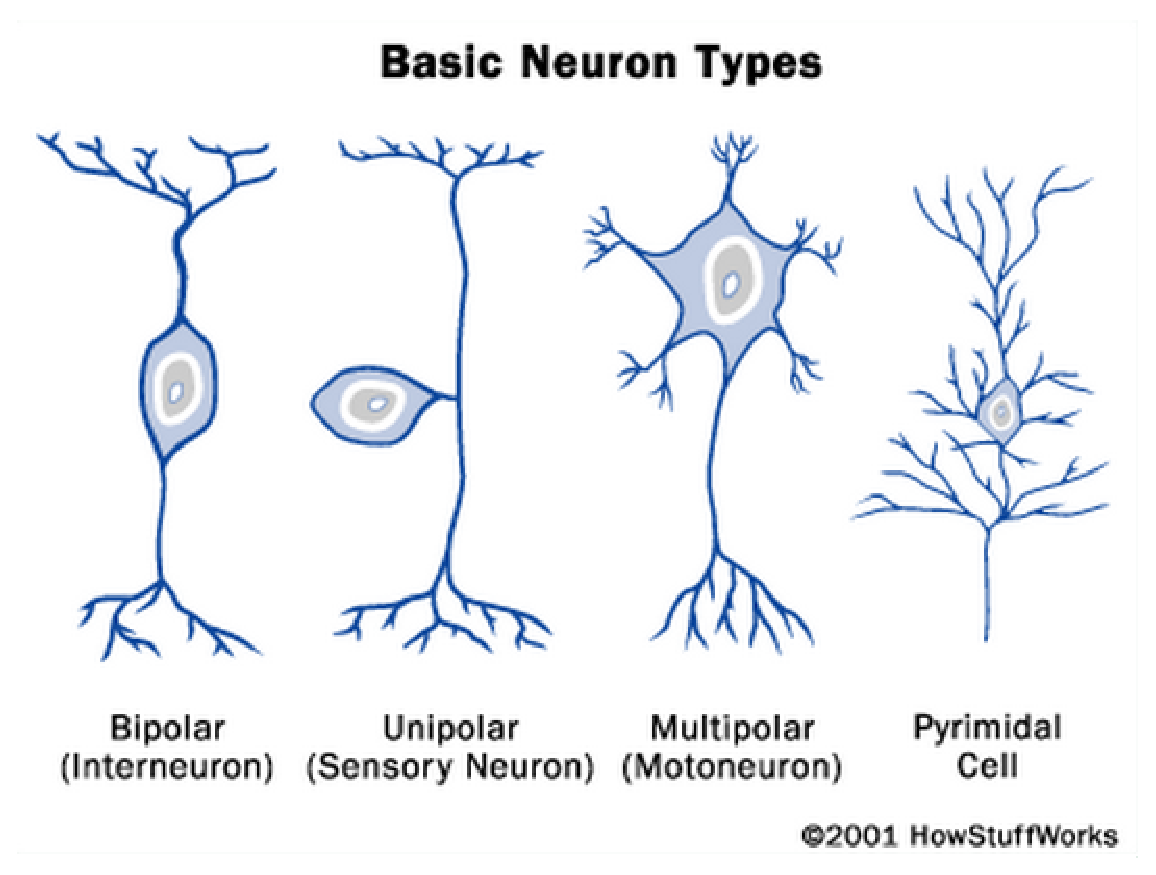
\includegraphics[height=7cm,
    angle=0]{./images/neuron_types.eps}}

  \centerline{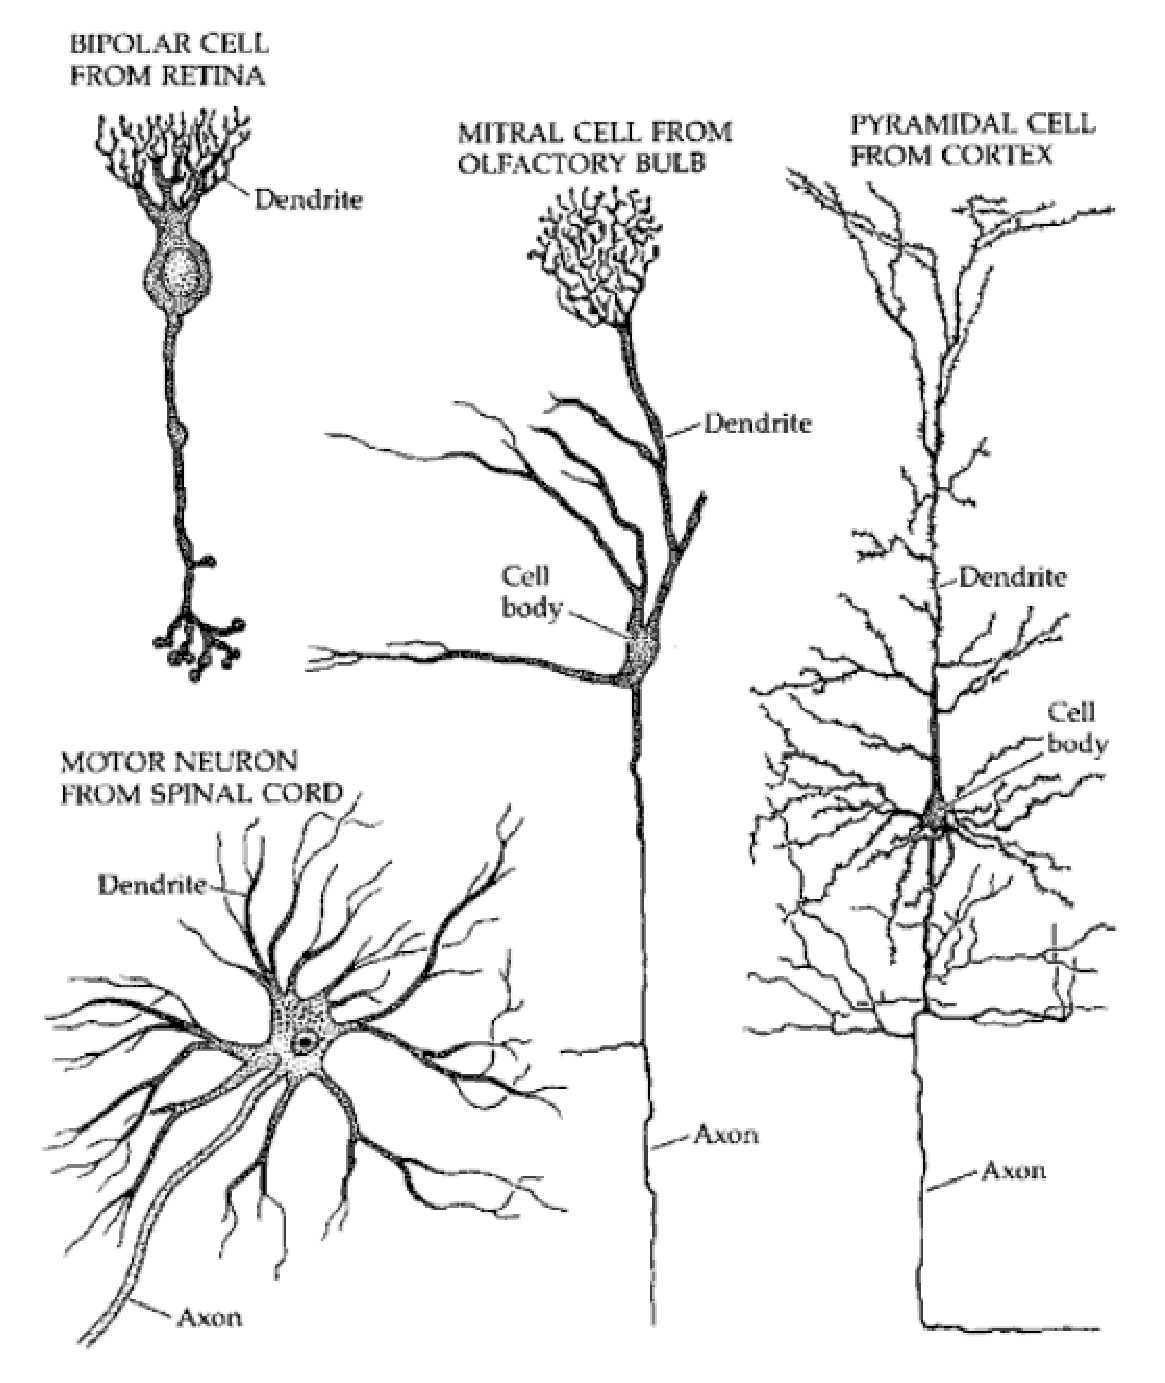
\includegraphics[height=7cm,
    angle=0]{./images/neurons.eps}
    %}, 
  %\centerline{
  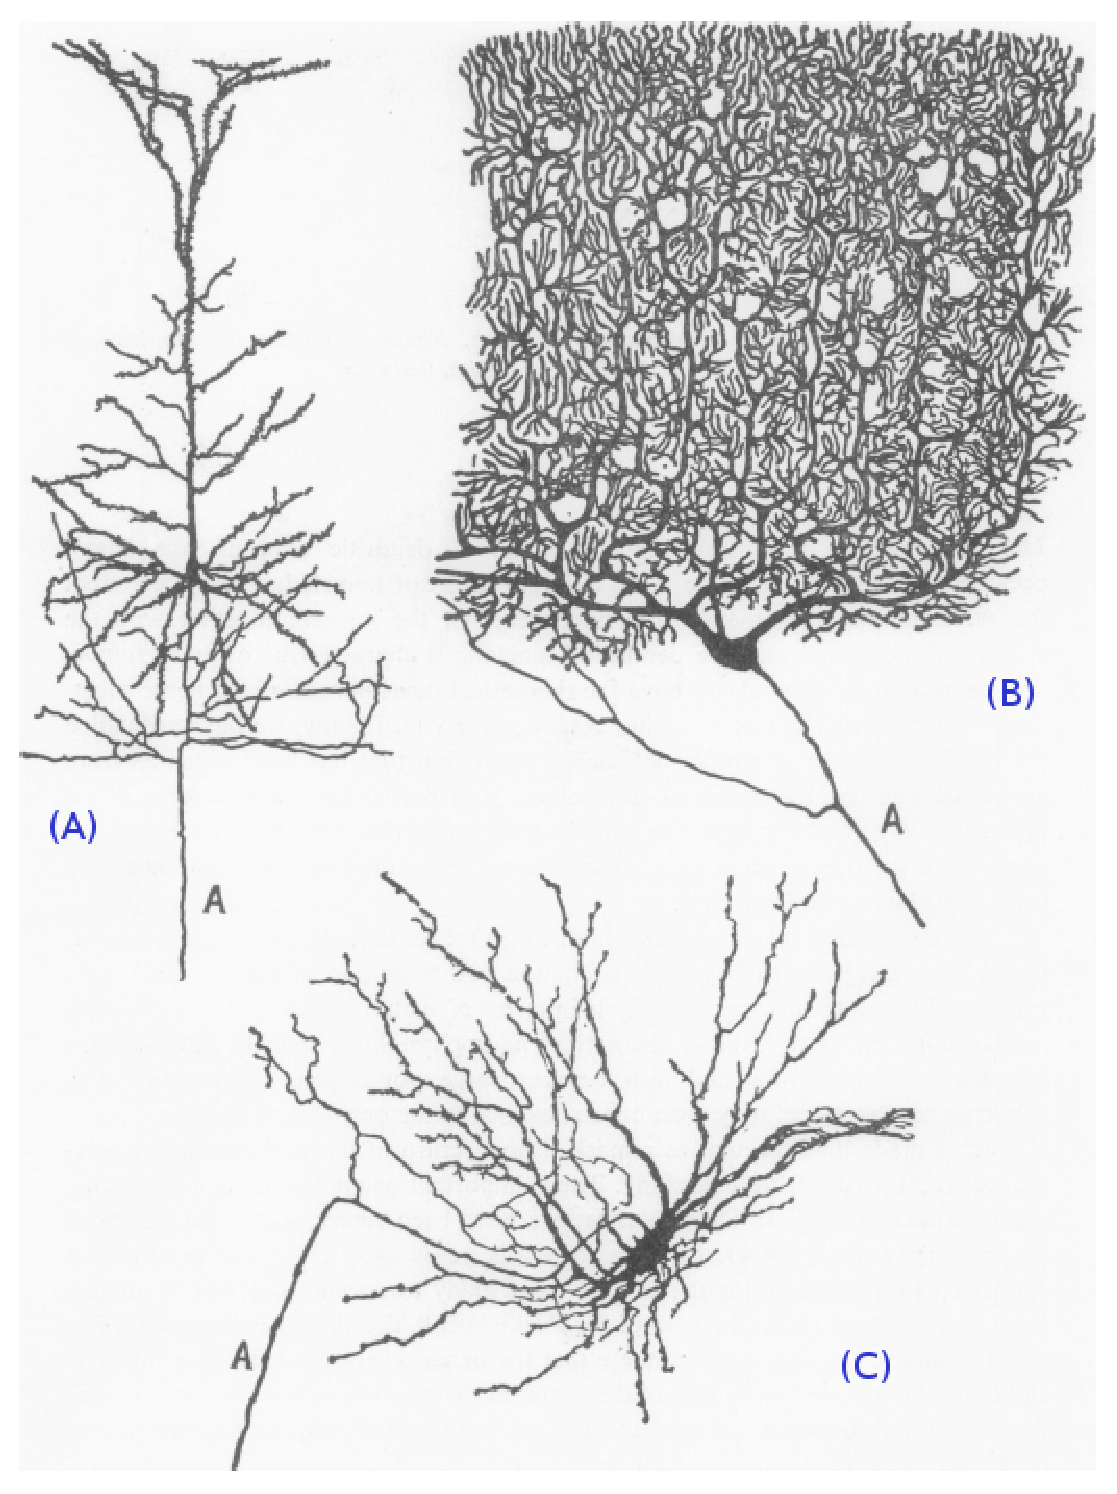
\includegraphics[height=7cm,
    angle=0]{./images/neuron_cells.eps}
    }
\caption{Different morphologies of neurons: (A) Pyramidal cell, (B) Purkinje
cell of cerebellum, (C) Motoneuron of spinal cord. NOTE: The letter 'A' means axon of the neuron}
\label{fig:neuron_cell}
\end{figure}


% \section{Introduction}
% \label{sec:introduction-1}
%\section{Neuron classification}
%\label{sec:neur-class}

\subsection{Option 4: firing pattern}
\label{sec:neuron-classify-spiking-fast-regular-bursting}
\label{sec:regular-spiking-pattern}
\label{sec:fast-spiking-pattern}
\label{sec:intrinsic-bursting-pattern}

In terms of signalling, the cells can be classified into 4 groups,
Fig.\ref{fig:neuron_APs} \citep{nowak2003}:
\begin{enumerate}
\item regular spiking (RS, tonic spiking): 

Example: interneurons in neurostriatum.

\item fast spiking (FS): some neurons are notable for their high firing rates

Example: some types of cortical inhibitory interneurons, cells in globus
pallidus, retinal ganglion cells, 50\% of inhibitory neurons in the neocortex.

\item continuously bursting (CB) or chattering (CH)

\item intrinsic bursting (IB)

\end{enumerate}

Excitatory neurons in the superficial layers tend to be
RS-type. Excitatory neurons in the deeper layers tend to be of both
RS- and IB- or CB- type. 

In many cases, bursting is not endogenous, but rather a condition that is
evoked under an injecting of a constant-current stimulus. Other figures:
Fig.\ref{fig:neural_firing_behavior}

\begin{figure}[hbt]
  \centerline{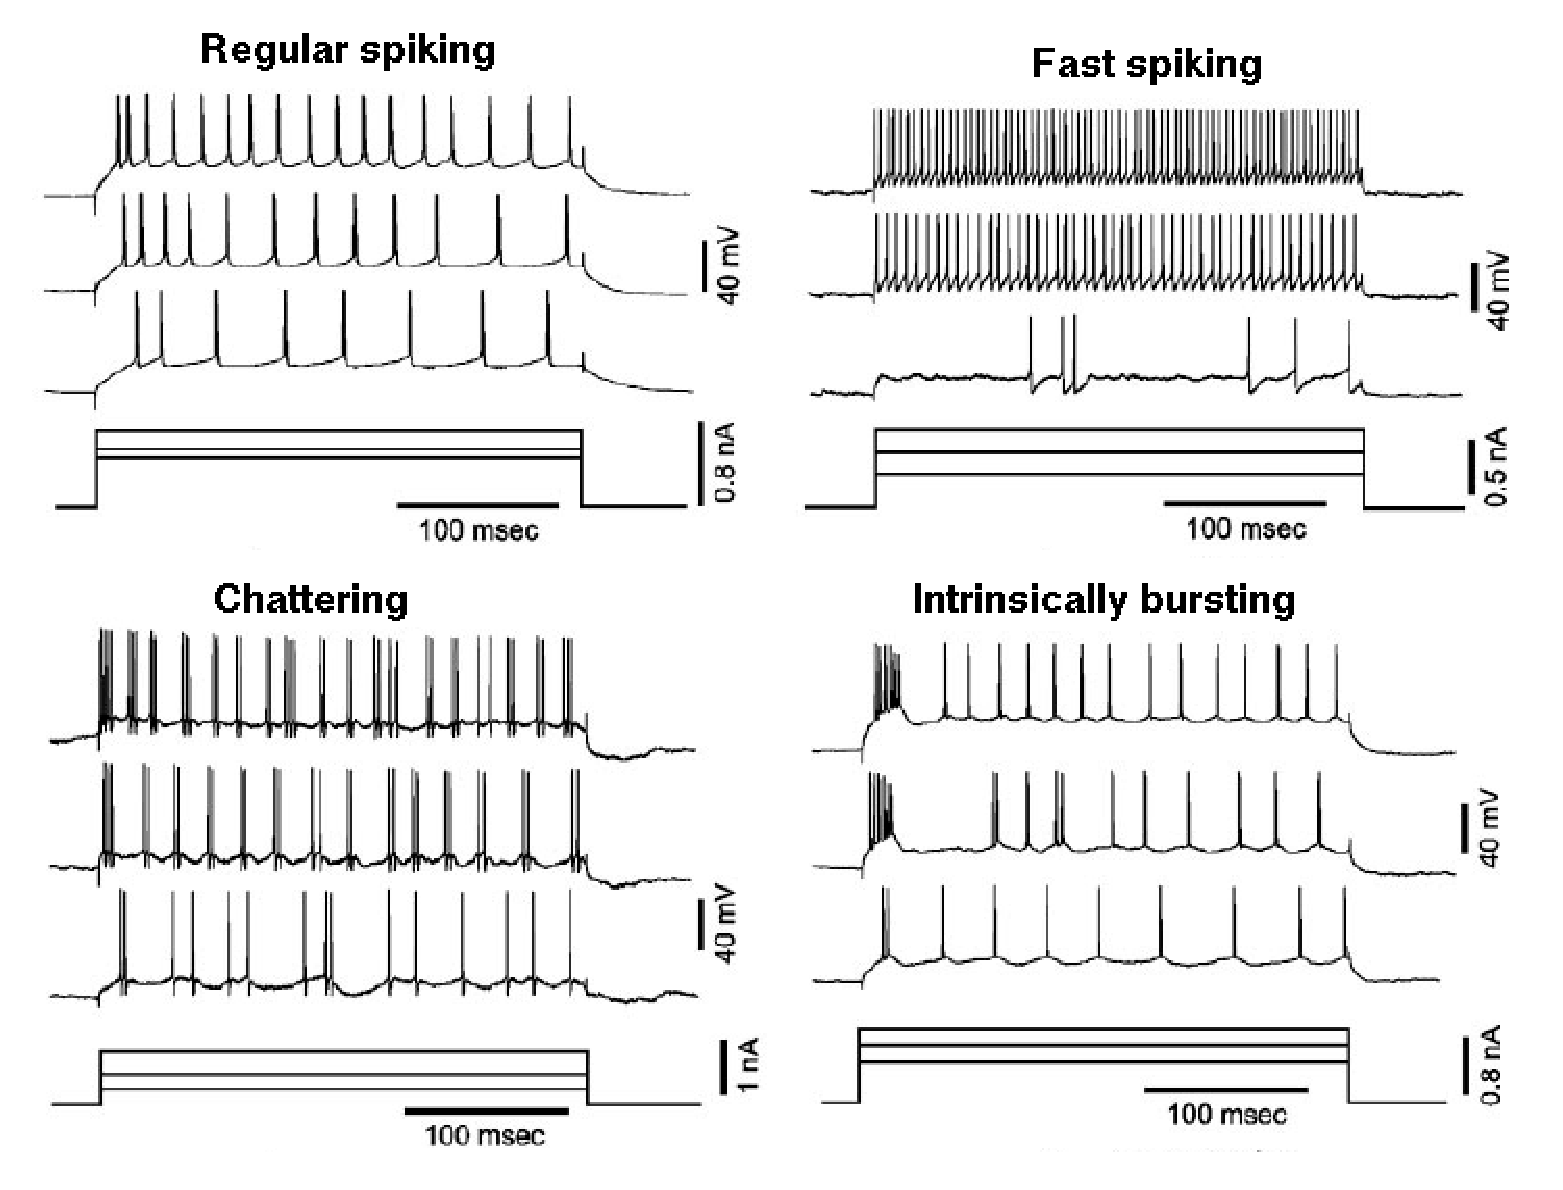
\includegraphics[height=7cm,
    angle=0]{./images/neuron_APs.eps}}
\caption{Examples of AP response to depolarizing current injection in 4
subjectively classified subtypes of cortical neurons: (RS), (FS), CH (CB), and
IB}
\label{fig:neuron_APs}
\end{figure}

\subsection{Option 5: group A, B, C}
\label{sec:neuron-classify-group-A,B,C}

\begin{itemize}
  \item group A cells: always myelinated, with high conduction velocity
  
  \begin{enumerate}
    \item A1-A7 cells: noradrenergic neurons (Sect.\ref{sec:noradrenergic-neurons})
    \item A8-A16 cells: dopaminegic neurons (Sect.\ref{sec:dopaminegic_neurons})
  \end{enumerate}
  \url{https://en.wikipedia.org/wiki/Nerve_fiber#Motor_fibers_of_the_A_group}
  
  \item group B cells: moderately myelinated, with conduction velocity 3-14 m/s
  \begin{enumerate}
    \item 
  \end{enumerate}
  \url{https://en.wikipedia.org/wiki/Group_B_nerve_fiber}
  
  \item group C cells: they are unmyelinated and have a small diameter and
  \textcolor{red}{low conduction velocity} (< 2 m/s); they are afferent neurons
  (Sect.\ref{sec:neuron-classify-afferent-efferent-inter})
  with average 0.2-1.5 $\mum$ diameter.
  
  \begin{enumerate}
    \item adrenergic cells - Sect.\ref{sec:adrenergic_neuron}
  \end{enumerate}
  \url{https://en.wikipedia.org/wiki/Group_C_nerve_fiber}
\end{itemize}


\section{Detecting neuron subpopulation in a type}

Determining whether a cell population is heterogeneous - whether it consists of
distinct sub-populations - is important for understanding cellular physiology
and identifying therapeutic targets.

Example: determine MSN is D1-MSN or D2-MSN.

Distinguishing MSNs while recording has been technically difficult and labor
intensive, requiring either single-cell gene profiling (Surmeier et al., 1996)
or axonal tracing (Kawaguchi et al., 1990).

Single-cell profiling, i.e. high-throughput analysis of individual cells using
technique such as flow cytometry.  While flow cytometry is effective, it is
limited by the availability of antibodies. Only a minority of known human genes
have commercially available antibodies. . Flow cytometry is also difficult to
perform when the distinguishing features of subpopulations are molecules inside
the cells rather than on the surface of cells.

Detecting intracellular features such as specific mRNA molecules does not
require antibodies and possesses enormous potential because it can exploit the
genomics and microarray data, i.e.  single cell mRNA abundance measurements are
required
\begin{enumerate}
  \item FISH - Sect.\ref{sec:FISH}
  \item RT-PCR - Sect.\ref{sec:RT-PCR}
\end{enumerate}




\section{Neuron types}
\label{sec:neuron-types}

In this section, we discuss different neuron types.
Sect.\ref{sec:neuron-type-classification} discusses different classification
systems.

\subsection{Cortical neurons}
\label{sec:cortical-neurons}

Cortical neurons refers to hundreds of different types of neurons in the
neocortex (Sect.\ref{sec:neocortex}). There are two broad classes of cortical
neurons:

\begin{enumerate}
  \item interneurons - Sect.\ref{sec:interneurons}
  
They can be basket cells (Sect.\ref{sec:basket-cell-cortex}).  
  
  \item projection neurons - Sect.\ref{sec:projection-neurons}
\end{enumerate}

\subsection{CSMN}
\label{sec:CSMN}

Corticospinal motor neurons (CSMNs) residing in cortical layer V of the
mammalian brain project their axons to the spinal cord, where they connect with
spinal motor neurons (SMNs) located in the ventral horn of the spinal cord.
\citep{mandemakers2014}.

CSMNs are of great interest because they form the basis of voluntary movement in
humans, they degenerate in degenerative motor neuron diseases including
amyotrophic lateral sclerosis (ALS), and their injury contributes to the loss of
motor function after spinal cord injury

\subsection{Adrenergic neurons}
\label{sec:adrenergic_neuron}

{\bf Adrenergic neurons} are those that release neurotransmitter epinephrine
(Sect.\ref{sec:epinephrine}).
They are nerve cells that show evidence of having phenylethanolamine
N-methyltransferase (PNMT), the enzyme that can convert norepinephrine to
epinephrine (Sect.\ref{sec:Catecholamines}).

\begin{itemize}
  \item C1 cells = found in conjunction with noradrenergic neurons group A1 in
  ventrolateral medulla (Sect.\ref{sec:noradrenergic-neurons})
  
  
  \item C2 cells = found in conjunction with noradrenergic neurons group A2 in
  dorsomedial medulla 
  
  \item C3 cells = found in conjunction with noradrenergic neurons group A3 in
  dorsal midline of rostral medulla (only found in rodent; but not in other
  species, including primates)
    
\end{itemize}
\url{https://en.wikipedia.org/wiki/Adrenergic_cell_groups}




\subsection{Basket cells}
\label{sec:basket-cell}

{\bf Basket cells} are GABAergic interneurons found in 
\begin{enumerate}
  \item the molecular layer of cerebellum:
  Sect.\ref{sec:basket-cell-cerebellum}.
  
  \item cortex: Sect.\ref{sec:basket-cell-cortex}
  
  \item hippocampus: Sect.\ref{sec:basket-cell-hippocampus}
\end{enumerate}

Basket cells are multipolar interneurons that function to make inhibitory
synapses and control the overall potentials of target cells due to its
axon-somata projection. The branched axonal arborizations give rise to the name
as they appear as baskets surrounding the soma of the target cell.

\subsection{-- cerebellum basket cells}
\label{sec:basket-cell-cerebellum}

Cerebellum basket cells are found  on the molecular layer of cerebellum
(Sect.\ref{sec:cerebellar_cortex}).
The dendrites of basket cells are free branching, contain smooth spines, and
extended from 12 to 30 mm, Fig.\ref{fig:cerebellum_greymatter}(B).
Basket cells have shown to form axo-somatic synapses on the cell bodies of
Purkinje cells (Sect.\ref{sec:Purkinjie_nerves}) and thus make inhibitory
effect on Purkinje cells.



\subsection{-- cortex basket cells}
\label{sec:basket-cell-cortex}

Basket cells (Sect.\ref{sec:basket-cell}) make up 15-25\% of total neurons in
the cortex (Sect.\ref{sec:neonatal-cells}).

3 types of basket cells in the cortex: small, large and nest type, that all are
interneurons that perform axo-somatic synapses
% % TODO COMPBIO: Understand the importance of axo-somatic synapse vs.
% axo-dendritic synapse
\begin{enumerate}
  
  \item small basket cell: short axon, and the axon of a small basket cell
  arborizes in the vicinity of that same cell's  dendritic range.
  
  \item large basket cell: the long axon innervate somata in different cortical
  columns
  
  \item nest basket cell: an intermediate form of the small and large cells,
  their axons are confined mainly to the same cortical layer as their somata
\end{enumerate}


\subsection{-- hippocampal basket cell}
\label{sec:basket-cell-hippocampus}

Basket cells in hippocampus form axo-somatic synapses and axo-proximal dendrites
of pyramidal neurons (Sect.\ref{sec:pyramidal-neurons}). 

Like their counterpart in the cortex (Sect.\ref{sec:basket-cell-cortex}),
hippocampal basket cells also are parvalbumin-expressing
(Sect.\ref{sec:parvalbumin-positive-interneuron}) and fast-spiking

\begin{itemize}

  \item in CA3 region: basket cells can form recurrent inhibition loops with
  pyramidal cells

\begin{verbatim}
basket cell A --[inhibit]---> pyramidal A ---[innervate]-->basket cell A
               --(loop back)--> pyramidal A
\end{verbatim}  
This closed loop can help dampen excitatory responses.

  \item 
\end{itemize}


\subsection{Cortical afferent neuron}
\label{sec:cortical-afferent-neuron}

{\bf Cortical afferent neurons} refer to cortical neurons.
Cortical afferent fibers are axonal terminal that projects to cortical neurons. 
%  Example of them are
% \begin{enumerate}
%   \item medium-sized spiny neuron in striatum
%   
%   \item \ldots
% \end{enumerate}

\subsection{Cortical efferent neuron}
\label{sec:cortical-efferent-neuron}

{\bf Cortical efferent neurons} refer to neurons that receives the input from
cortical neurons. Example of them are
\begin{enumerate}
  \item medium-sized spiny neuron in striatum

Layer V gives rise to all of the principal cortical efferent projections to
basal ganglia MSN.
  
  \item \ldots
\end{enumerate}



\subsection{Cajal-Reizius cells}
\label{sec:Cajal-Reizius-cell}

These cells were discovered by two scientists, Cajal and Retzius, at two
different times and in different species. 
They release {\it reelin} (Sect.\ref{sec:reelin}).

Nowadays, the name refers to a heterogeneous population of morphologically and
molecularly distinct reelin-producing cell types found in the marginal zone of
layer I neocortex (Sect.\ref{sec:layer-I}). The cells laid closer to the pia and
displayed smaller, often triangular or pyriform somata, and less complex
processes that lacked the ascending branchlets and had a more superficial
location than the cells Retzius previously described

\subsection{Chandelier cells}
\label{sec:chandelier-cells}

Chandelier neurons or chandelier cells are a subset of GABA-ergic cortical
interneurons.  The name comes from the specific shape of their
axon arbors
\begin{itemize}
  \item axon terminals forming distinct arrays called "cartridges"
  (Sect.\ref{sec:synapse-types}).
  
  \item GAT-1 is the isoform of the GABA membrane transporter found
  (Sect.\ref{sec:GABA-vesicular-transporter}).
  
  \item Chandelier neurons synapse exclusively to the axon initial segment of
  pyramidal neurons of cortex, near the site where action potential is generated
  
It is believed that they provide inhibitory input to the pyramidal neurons, but
there is data showing that in some circumstances the GABA from chandelier
neurons could be excitatory [Szabadics et al., (2006) - Science].
% Szabadics, J.; Varga, C.; Molnar, G.; Olah, S.; Barzo, P.; Tamas, G. (2006).
% "Excitatory Effect of GABAergic Axo-Axonic Cells in Cortical Microcircuits".
% Science. 311 (5758): 233-235. 
  
\end{itemize}

It has been belived that chandelier neurons are parvalbumin-positive
interneurons; though  more recent work has suggested that only a subset of
chandelier cells test positive for parvalbumin by immunostaining [Taniguchi et
al., (2013) - Science].
% Taniguchi H, Lu J, Huang ZJ (January 2013). "The Spatial and Temporal Origin of
% Chandelier Cells in Mouse Neocortex". Science. 339 (6115): 70-4.




\section{Catecholaminergic neurons}
\label{sec:catecholaminergic-neurons}

Catecholaminergic neurons are those that contain either the neurotransmitters
dopamine (dopaminergic system) or norepinephrine (noradrenergic system). These
neurons are estrogen-sensitive, and brainstem catecholaminergic neurons contain
small numbers of intracellular ER (McEwen and Alves, 1999). 
 
 
 The enzyme tyrosine hydroxylase is the rate-limiting step in the conversion of
 L-tyrosine to L-DOPA in the synthesis of dopamine and then norepinephrine, and
 estradiol regulates tyrosine hydroxylase gene expression in catecholaminergic
 neurons.
 
 
 
  
\subsection{(Large aspiny) Cholinergic neurons (ChAT)}
\label{sec:cholinergic_neurons}
\label{sec:ChAT-expressing-neuron}

Cholinergic neurons are neurons that release acetylcholine
(Sect.\ref{sec:Acetylcholine}) as neurotransmitters upon activation. They are
very important in muscle contraction, memory, and learning.

The cholinergic interneurons are giant aspiny neurons (with a somatic diameter
that can be in excess of 40 $\mum$) expressing the {\bf choline
acetyltransferase} (ChAT; Kawaguchi et al., 1995). ChAT is responsible for the
synthesis of neurotransmitter acetylcholine, from CoA (Sect.\ref{sec:CoA}).
 ChAT is found in high concentration in cholinergic neurons, both in the central
nervous system (CNS) and peripheral nervous system (PNS). ChAT is produced in
the body of the neuron and is transported to the nerve terminal, where its
concentration is highest. Presence of ChAT in a nerve cell classifies this cell
as a "cholinergic" neuron.




They are found in
\begin{enumerate}
  \item {\bf basal forebrain}: Unlike cholinergic neurons in striatum, the
  forebrain cholinergic neurons do not contain D2-receptor mRNA
  \citep{lemoin2014}.
  
  

The primary concentration of cholinergic neurons/cell bodies that project to the
neocortex are in the basal nucleus of Meynert (Sect.\ref{sec:nucleus-basalis})
in basal forebrain - Sect.\ref{sec:basal-forebrain}.

Acetylcholine is known to promote wakefulness in the basal forebrain.
Stimulating the basal forebrain gives rise to acetylcholine release, which
induces wakefulness and REM sleep, whereas inhibition of acetylcholine release
in the basal forebrain by adenosine causes slow wave sleep.


Adenosine acts on A1 receptors (Sect.\ref{sec:A1A-receptor}) of cholinergic
neurons in the basal forebrain. This results in hyperpolarization of cholinergic
neurons, which inhibits the release of acetylcholine.

  \item {\bf putamen of striatum}: 

Striatal cholinergic interneurons are implicated in motor control, associative
plasticity, and reward-dependent learning. In striatum, 80\% of cholinergic
neurons in the striatum contain detectable D2 receptor mRNA. 

Synchronous activation of cholinergic interneurons triggers large inhibitory
synaptic currents in dorsal striatal projection neurons, providing one potential
substrate for control of striatal output, but the mechanism for these GABAergic
currents is not fully understood. In rhesus monkey, all examined neurons of
large size of cholinergic interneurons (mean diamater 26.1$\mum$) were
moderately labeled for GluR1 - Sect.\ref{sec:AMPAR-distribution} (Deng, Reiner,
2010).

\label{sec:IMTC-technique}
\label{sec:immunotoxin-mediated-cell-targeting}
Cholinergic interneurons are identified using a classical additional
transgenesis by Nakanishi and colleagues in 2000.
They ablated the neurons by {\bf immunotoxin-mediated cell targeting (IMTC)}
which allows a conditional and time controlled destruction of neurons (Kaneko et
al., 2000). A transgene was made containing the alpha subunit of human
interleukin-2 receptor (hIL-2R$\alpha$) under the control of the mouse 18.3 kb
5'-upstream genomic sequence containing the first and second exons of the mGluR2
gene.

\end{enumerate}




\subsection{Dopaminegic neurons}
\label{sec:dopaminegic_neurons}


{\bf Dopaminergic neurons}: a neuron that upon stimulation (activation) release
dopamines (DA - Sect.\ref{sec:dopamine}) as the neurotransmitters. The neurons' soma
produce the enzymes that synthesize dopamine. Make sure you know about catecholamine
(Sect.\ref{sec:Catecholamines}), especially dopamine (Sect.\ref{sec:dopamine}).
 
Dopaminergic neurons are found in many regions; but mainly concentrate in two
areas of the brainstem: 
\begin{enumerate}
  \item  the {\it substantia nigra pars compacta} (SNpc)
  (Sect.\ref{sec:substantia_nigra}) and 

DA neurons in SNpc (Sect.\ref{sec:SNpc}) tend to be melanin-pigmented due to the
presence of black pigment melanin.
  
  \item the ventral tegmental area (VTA) in the midbrain
  (Sect.\ref{sec:ventral-tegmented-area}), which is DA-rich and contains both redox available
  neuromelanin and a high iron content. 
  
\end{enumerate}
In mouse olfactory bulb - Sect.\ref{sec:olfactory-nerve}.

Dopaminergic SNpc and VTA neurons differ on several functional levels, and
dopaminergic SNpc neurons themselves vary in their intrinsic electrical
properties, neurochemical characteristics and connections.

Firing of SNpc dopaminergic neurons is brain state-dependent, and, unlike
VTA dopaminergic neurons, they are not commonly recruited or inhibited by
aversive stimuli (Brown et al, 2009).

\begin{enumerate}
  \item calbindin-positive DA neurons in the SNpc that also innervate the
  striatum
  
Calbindin (CB) expression by some dopaminergic SN neurons has been linked with
their increased survival in Parkinson's disease.
  
  \item DA neurons in VTA innervate NAc (ventral striatum)
  \item DA neurons in SNpc innervate dorsal striatum
\end{enumerate}

\begin{mdframed}

According to the nomenclature of Dahlstrom and Fuxe (1964), DA cells generally
corresponds to A9 area of the substantia nigra (SN), A10 area of ventral
tegmental area (VTA), and the retrorubral area (A8) (Berger et al, 1991; Porrino and
Goldman-Rakic 1982; Williams and Goldman-Rakic, 1998)
%  NOTE: Dopaminergic neurons
% in the SNpc


\begin{itemize}
  \item A8 cells = a small group of dopaminergic neurons found in (1) in mouse
  at in the retrorubral field, (2) in rodents and primates at reticular
  formation dorsolateral to the substantia nigra

  \item A9 cells = the {\bf most densely packed group} of dopaminergic neurons
  located in the ventrolateral midbrains in rodents and primates which is {\it
  for the most part identical to} the substantia nigra pars compacta
  (Sect.\ref{sec:SNpc}).
  

  \item A10 cells = the {\bf largest group} of dopaminergic neurons, located for
  the most part in the VTA (Sect.\ref{sec:ventral-tegmented-area})
  
  \item A11 cells = a small group \ldots
  
  \item A12 cells =  a small group of dopaminergic neurons in arcuate nucleus of
  the hypothalamus and the immediate periventricular nucleus
  
  \item A13 cells = 
  
  \item A14 cells = 
  
  \item A15 cells = 
  
  \item A16 cells = found in the olfactory bulb of vertebrates (including
  rodents and primates)
\end{itemize}
\url{https://en.wikipedia.org/wiki/Dopaminergic_cell_groups}
\end{mdframed}


\textcolor{red}{DA neurons are unique in that their axon can emanate from a
primary dendrite rather than directly from the soma as is usually the case in
other
neurons}.\footnote{\url{http://www.scholarpedia.org/article/Dopamine_anatomy}}
DA neurons are expected to involve in higher motor execution and goal-directed
behavior, including motivation, reward learning and prediction, and working
memory, rather than in basic sensory processes.

DA axons can form both symmetric (type II) and asymmetric (type I) synaptic
contacts (Sect.\ref{sec:synapse-symmetric}), although the latter ones clearly
represent a minority (3-22\% of all DA synapses, where the variability may stem
partly from differences in methodology (see Smiley and Goldman-Rakic, 1993 for a
discussion of technical considerations) and partly from the area investigated,
e.g. Descarries et al, 1987; Segula et al, 1988)

\textcolor{red}{Axon projection}
\begin{enumerate}
  \item the basal ganglia, in particular the striatum, receive by far the
  densest dopaminergic input.
  
  \item Within the neocortex,  a relative paucity of dopaminergic inputs to
  primary sensory areas (like primary visual cortex V1), while motor cortical,
  prefrontal (especially orbitofrontal) and anterior cingulate areas are among
  the most densely innervated.
  
  {\it Layer-specific patterns of innervation}:
  In the rat prefrontal cortex, the deep layers V-VI receive the strongest DA
  input while in primates superficial layers I-III are at least as densely
  innervated.
\end{enumerate}
The axon projections of DAergic neurons can be classified into four major
dopaminergic pathways that have been identified in the mammalian brain
(Sect.\ref{sec:dopaminegic_pathways}).

\subsection{-- DA release}

Low level of DA release have been correlated with low frequency firing rate of
DA neurons (somata located in either VTA or SNc), while corresponding
enhancement in striatal DA release occurs in response to high frequency firing
rates (Kawagoe et al., 1992). 

BUT, recent evidences also suggest that DA release not necessarily require DA
neuron firing, i.e. local control factors such as reuptake
(Sect.\ref{sec:DA-reuptake}), autoreceptor-dependent modulation,
termino-terminal control.

\begin{enumerate}
  \item firing of DA neurons increase in the midbrain (Sect.\ref{sec:midbrain})
  in response to rewarding stimuli in non-human primates (Schultz et al., 1997; Schultz, 1998)
  
 fMRI studies in human points to a similar
 increase in cellular activity (D'Ardenne etal., 2008)

  \item 
\end{enumerate}

\subsection{-- DA reuptake (DA transporter)}
\label{sec:DA-reuptake}
\label{sec:DA-transporter}

After the release of DA from the vesicles into the synaptic cleft, reuptake by
the {\bf dopamine transporter} (DAT) in the presynaptic membrane occurs after
which the DA is transported back into vesicles or is degraded to DOPAC by type B
monoamine oxidase (Olivier et al., 2000; Shih et al., 1999).

The time course and local specificity of its action depend to a large extent on
the regionally specific properties of uptake/breakdown of DA
\begin{itemize}
  
  \item  In limbic and cortical regions such as the basolateral amygdala and
  PFC, {\bf DA clearance rates are slower than in the striatum} (Cass and
  Gerhardt 1995; Garris et al, 1993, Garris and Wightman, 1994).
  
  Unlike in striatal regions, the PFC shows very low levels of DA transporter
  expression (Sesack et al, 1998), and the DA transporter accounts for only ~
  40\% of DA uptake in the PFC, compared with ~ 95\% in the striatum (Wayment et
  al, 2001).
  
  In PFC, a significant portion of DA uptake is mediated by the
  norepinephrine transporter and catabolized enzymatically by
  catechol-O-methyltransferase and to a lesser degree monoamine oxidase (Cass
  and Gerhardt 1995; Moron et al, 2002; Wayment et al, 2001).
  
\end{itemize}

\subsection{-- DA function}

Brain DA
\begin{enumerate}
  \item bind to DA-receptors (Sect.\ref{sec:dopamine_receptors})
  
  
  \item modulate the efficacies of 
  \begin{enumerate}
    \item NMDAR
    
Review: \citep{cepeda2009} in the striatum.
 DA modulation of spontaneous or glutamate-induced action potentials in the
 caudate nucleus of striatum has been known for some time.
Recent studies revealed the presence of physical interactions between NMDA and
DA receptors at the membrane and cytoplasm levels.
    
    \item some types of $\Ca$ channels ???
    
    \item $\Na$ channels
    \item $\K$ channels 
  \end{enumerate}
  which means it affects the bacpropagation of AP
  (Sect.\ref{sec:back-propagating_AP}).
\end{enumerate}


Dysfunction of brain DA has been linked to a variety of neuropsychiatric
disorders \citep{emilien1999}
\begin{enumerate}
  \item Schizophrenia [18] - Sect.\ref{sec:schizophrenia}
  
  \item social phobia,[17] 
  
  \item Tourette's syndrome,[18] 
  
  \item Parkinson's disease,[19]

A deficiency of dopamine in these ganglia leads to parkinsonism, and this
deficiency is at least partially alleviated by the administration of L-dopa.
  
  \item neuroleptic malignant syndrome,[20] 
  
  \item attention-deficit hyperactivity disorder (ADHD),[21] and 
  
  \item drug and  alcohol dependence.
  
\end{enumerate}



\subsection{Enkephalin-containing neurons}
\label{sec:enkephalin-containing-neurons}
\label{sec:ENK-containing-neurons}

Enkephalins (ENK) are endogenous opiates that are assumed to modulate
nociceptive information by mediating synaptic transmission in the central
nervous system, including the spinal dorsal horn.

Enkephalin-containing neurons are found in
\begin{itemize}

  \item D2-MSN in striatum - Sect.\ref{sec:iSPN-vs-dSPN}
  
  
  \item the dorsal horn of the spinal cord, where they play an
important role of modulation nociceptive information.

Enkephalinergic neurons express 5-HT$_3$ receptors
(Sect.\ref{sec:5-HT3-receptor}) in the dorsal horn of the spinal cord.
Activation of 5-HT3 receptors facilitates GABA release from some interneurons in
SD
  
\end{itemize}

\subsection{Granule cells}
\label{sec:granule_cells}

The majority of granule cells are in dentate gyrus
(Sect.\ref{sec:dentate_gyrus}). They are also found within the deep granular
layer of the cerebellum (Sect.\ref{sec:cerebellum}), the superficial layer of
the dorsal cochlear nucleus, the olfactory bulb, and the cerebral cortex
(Sect.\ref{sec:layer-IV}).
Granule cells in different brain regions are both functionally and anatomically
diverse: the only thing they have in common is smallness.
\begin{enumerate}
  \item cerebellar granule neurons - Sect.\ref{sec:cerebellar-granule-neuron}
\end{enumerate}

Granule cells release glutamate as neurotransmittes. The mechanism of release
changes over time \citep{gallo1982}
% gallo et al (1982) Selective release of glutamat from cerebellar granule cells
\begin{itemize}
  \item in fetal calf of 2 days in vitro: the newly synthesized glutamate evoked
  by high $[\K]$ and is $\Ca$ independent
  
  \item at later stages (4,8 to 12 days in vitro): it becomes $[\Ca]$ dependent
  heavily
\end{itemize} 

The rapid release comes in two phases
\begin{enumerate}
  \item rapid release that occurs within a few milisecond of the neuron's spike
  \item a more sustained elevation of release probability (i.e. delayed
  release):

The study of synapse between cerebellar granule cell and postsynaptic target
(stellat cells and Purkinje cels) showed that the delayed release is splited
into 2 phases \citep{atluri1998} (Atluri - Regehr, 1998)
\begin{itemize}
  \item one lasting 10s of miliseconds: steeply $\Ca$-dependent
  \item one lasting 100s of miliseconds: driven by low levels of $\Ca$ with
  nearly linear $[\Ca]$-dependency
\end{itemize}

The steep calcium dependence of delayed release, combined with the large calcium
transients observed in these presynaptic terminals, suggests that for
physiological conditions delayed release provides a way for cells to influence
their postsynaptic targets long after their own action potential activity has
subsided.


\end{enumerate}

\subsection{GABAergic neurons}
\label{sec:GABAergic-neurons}

GABAergic neurons are inhibitory neurons (Sect.\ref{sec:inhibitory-cell}) that
upon activated, the neuron releases GABA neurotransmitters, and the released
GABAs as inhibitory agent bind to GABA receptors on the postsynaptic neurons
(Sect.\ref{sec:GABA_receptors}).

To detect these neurons, we can use
\begin{enumerate}
  \item GABAergic marker: Glutamic Acid Decarboxylase (GAD) - Sect.\ref{sec:GAD}
  
  \item 
\end{enumerate}

Example of GABAergic neurons:
\begin{itemize}
  \item Purkinje neurons - Sect.\ref{sec:Purkinjie_nerves}

  \item Medium-sized spiny neuron (striatal projection neurons) -
  Sect.\ref{sec:medium_spiny_neurons}

  \item Striatal Fast-spiking interneuron -
  Sect.\ref{sec:fast-spiking-interneuron}

  \item Cortical interneurons - Sect.\ref{sec:cortical-interneuron}
  

\end{itemize}






\subsection{GAD-positive (inter)neuron}
\label{sec:GAD-positive-neuron}

GAD-positive interneuron is just different name refering to
GABAergic neurons - Sect.\ref{sec:GABAergic-neurons}, as these neurons are
detected using GAD as the marker (Sect.\ref{sec:GAD}). 

 




\subsection{Glutamatergic neurons}
\label{sec:glutamatergic_neurons}

Glutamatergic neurons are neurons that are excited by receiving glutamate
(Sect.\ref{sec:Glutamate}) from other neurons at the synapse called
glutamatergic synaptic junctions. The postsynaptic side of the synapse, i.e. the
side at glutamatergic neurons, have glutamate receptors
(Sect.\ref{sec:glutamate_receptor}).

The below neurons are glutamate neurons  
\begin{itemize}
  \item projection neurons - Sect.\ref{sec:projection-neurons} found in
  isocortex
  
  \item 
\end{itemize}

Check Sect.\ref{sec:synapse-activation} for different types of synapse
activation
\begin{itemize}
  
  \item Upon neurotransmitter released, which cause NMDAR opening, yet very few
  ions flow through the channel due to $\Mg$ blocking, which prevents ions from
  passing freely though the channel. Under such condition, the EPSP is mediated
  entirely by AMPAR.

At resting membrane potentials, external magnesium ($\Mg$) ions enter the NMDAR
pore, but unlike the permeant $\Ca$ ions, they bind tightly and prevent further
ion permeation. $\Mg$ ions are present at millimolar concentrations in the
external milieu of neurons, while intracellular $\Mg$ concentrations are in the
micromolar range, resulting in a net inward driving force for $\Mg$ ions at
negative membrane potentials.

NMDARs activate significantly slower than AMPARs and kainate
receptors. Because NMDARs have relatively a high affinity for glutamate, the
millisecond-long neurotransmitter pulses should be able to partially (and
slowly) activate NMDARs. However, individual excitatory synaptic inputs received
during baseline activity do not result in calcium ($\Ca$) influx because of a
second NMDAR property: its pronounced voltage dependence.

Activation of AMPARs is fast and transient, causing brief depolarizations that
last no longer than a few milliseconds.

  \item If the stimulus is of sufficient strength, AMPAR can help depolarize the
  postsynaptic membrane enough to expel $\Mg$ block from NMDAR.
  A depolarization of sufficient amplitude and duration is required to dislodge
  and repel the $\Mg$ ions from the pore. \textcolor{red}{There are several
  ways to achieve strong depolarization, which will be covered shortly}.
  
Now, unblocking NMDAR can actively response to glutamate, admitted not only
$\Na$ but also a large amount of $\Ca$.
The increase in postsynaptic [$\Ca$] can in turns function as a second messenger
in vaious signalling cascades, e.g. trigger the activation of CaMKII or trigger
the increase of neurotransmitter release via retrograde signal,
Fig.\ref{fig:Calcium-dendritic-spine}.
\begin{itemize}
  
  \item $\Ca$ bind to calmodulin, activate CaMKII. CaMKII phosphorylate AMPAR
  and making them more permeable to the inflow of $\Na$ ions (i.e. increase
  AMPAR sensitivity to depolarization) and in time, CaMKII can promotes the
  movement of AMPAR from the intracellular stores to the postsynaptic membranes,
  i.e. making more AMPAR availables to stimulate the dendritic spine.

The expression of new AMPA receptors takes place over 1-2 hours after LTP stimulated.

  \item  [This is still controversal] The increase of neurotransmitter release
  from the presynaptic axonal terminal via {\bf retrograde signal}, e.g. nitric oxide (NO) is release by the
  postsynaptic dendrite and travel 'backward' across the chemical
synapse to bind the axonal terminal of the presynaptic neuron which creates a
feedback loop.
\url{http://en.wikipedia.org/wiki/Retrograde_signaling}
\end{itemize}
\end{itemize}

\begin{figure}[htb]
\centerline{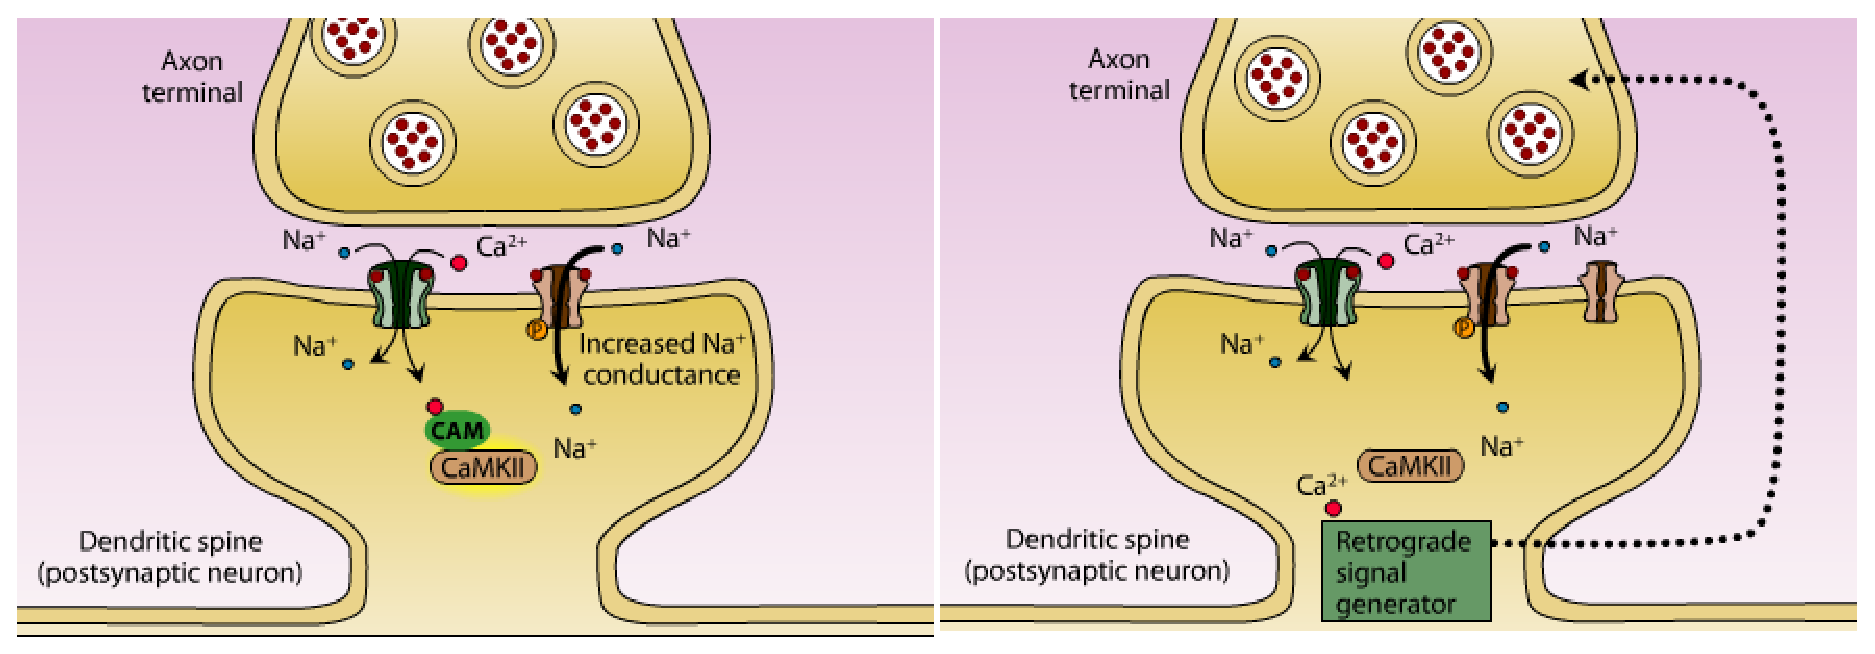
\includegraphics[height=4cm]{./images/Calcium-dendritic-spine.eps}}
\caption{(A) $\Ca$ trigger CaMKII; (B) $\Ca$
move to presynaptic axonal terminal via
retrograde signal}\label{fig:Calcium-dendritic-spine} 
%http://www.sumanasinc.com/webcontent/animations/content/receptors.html
\end{figure} 

{\bf METHODS TO ACHIEVE STRONG DEPOLARIZATION}:
\begin{enumerate}
  \item  High frequency synaptic inputs: allows the EPSP generated by AMPAR
  to accumulate and build up over time. This phenomenon underlie long-term
  potentiation (LTP) - Sect.\ref{sec:LTP}.

% Mechanism: During tetanus, the $\Mg$ block is removed from NMDA receptors,
% allowing larger PSP and allowing Ca2+ to enter the cell, activating other
% mechanisms.
NMDA receptors (Sect.\ref{sec:glutamate_receptor}) account for {\it specificity}
(LTP occurs only at synapses that are actively receiving glutamate at their NMDA
receptors), {\it state-dependence} (depolarization removes $\Mg$ block), and
{\it associativity} (input from one synapse may remove the $\Mg$ block at
another synapse that receives weak input).

NMDA antagonists block LTP without blocking regular PSPs. 

  \item Back-propagating action potential (bAP), i.e. the AP initiated from the
  axon actively backpropagate into the dendrites (in many neuronal types),
  providing a retrograde signal of neuronal output to the dendritic tree
  \citep{stuart1997} (Sect.\ref{sec:back-propagating_AP}. 
  
  Dendritic bAPs have a longer duration than axonal spikes and therefore permit
  the removal of $\Mg$ block from NMDARs. Any glutamate release occurring during
  a bAP-induced depolarization may therefore result in $\Ca$ influx through
  activated NMDARs and subsequent alterations in synapse strength.
  Because bAPs take time to propagate down distal dendrites, efficient
  activation of NMDARs by this mechanism requires precise timing of synaptic
  input relative to bAP generation.
   So, \textcolor{red}{this has to be at the right time between bAP and
  EPSP}. \citep{markram1997} found that the window (i.e. time gap) between bAP
  and EPSP within 10 ms. The precise timing between presynaptic firing and
  postsynaptic firing has given rise to a model of long-term synaptic plasticity
  called {\bf spike-timing dependent plasticity} (Sect.\ref{sec:STDP}).
  
\end{enumerate}

\subsection{GnRH-expressing neurons}
\label{sec:GnRH-expressing-neurons}

{\bf GnRH-expressing neurons} are found scattered throughout the hypothalamus
(Sect.\ref{sec:hypothalamus}), and produced from stem cells in the nasal tissue
and migrate into the brain along olfactory axon fibers from the nose.

GnRH neurons that fail to enter the brain, or that migrate to the wrong region,
are not functional and can even undergo programmed cell death.
This failure of GnRH neurons to migrate into the brain is the main cause of
Kallmann Syndrome.


Guidance molecules:
\begin{itemize}
  \item GABA depolarize the embryonic GnRH neurons; i.e. slow the movement but
  help the neurons move on the right path
  
  \item SDF activates hyperpolarizing GIRK channels which activate upon
  hyperpolarization, and accelerate the movement
  
  \item regulate the movement: Semaphorine, HGF
\end{itemize}

How the cell move?
\begin{itemize}
  \item normally, $\Ca$ are rapidly sequestered into organelles like
  mitochondria, ER
  
  \item guidance molecules above cause the release of $\Ca$ back into the
  cytoplasm, and $\Ca$-sensing proteins cause the contraction of the cells
  (similar to muscle contraction) that link to adhesive protein on the cell
  surface, pulling the cell forward.
\end{itemize}

In the hypothalamus, GnRH neurons receive input from classical neurotransmitters
like glutamate and GABA. The strongest activator of GnRH neurons is a hormone
called Kisspeptin.  GnRH neurons also integrate information from the body
through hormones like Neuropeptide Y (Sect.\ref{sec:neuropeptide-Y}) and
Adiponectin.

This triggers the release of GnRH into the hypophyseal
portal capillary bloodstream, where the GnRH hormone activates the pituitary to
release luteinizing hormone (Sect.\ref{sec:luteinizing-hormone}) and follicle
stimulating hormone (Sect.\ref{sec:FSH}).



\subsection{Grid cell}
\label{sec:grid-cell}

A grid cell is a type of neuron in the brains of many species that allows them
to understand their position in space. Two scientits discovered grid cells were
given Nobel Prize in 2014, together with John O'Keefe on a different type of
cell - place cell (Sect.\ref{sec:place_cells}).




\subsection{Histamine neurons}
\label{sec:histamine-neurons}

Histamine neuron are found only in the tuberomammillary nucleus, i.e. the sole
source of histamine, and the neurons project to 
\begin{itemize}
  \item NAc (Sect.\ref{sec:nucleus_accumbens})
\end{itemize}


\subsection{Intratelencephalic neurons}
\label{sec:Intratelencephalic-neurons}

{\bf Intratelencephalic corticostriatal projection neurons (CStrPNi)} (or
intratelencephalic (IT) cortical cells) are located predominantly in layer V of
the cerebral cortex (Sect.\ref{sec:cerebral_cortex}).
\subsection{Interneurons (relay neurons, association neurons, local circuit
neurons)}
\label{sec:interneurons}
\label{sec:relay-neurons}


Broadly speaking, {\bf interneurons} are neurons that connects afferent neurons
(Sect.\ref{sec:afferent_neurons}) and efferent neurons
(Sect.\ref{sec:efferent_neurons}). Interneurons are neither motor nor sensory
(Sect.\ref{sec:neuron-classify-afferent-efferent-inter}).

The neurons of the central nervous system (CNS), including the brain, are all
interneurons. However, in CNS, the term interneuron is widely used to refer to
small, locally projecting neurons (in contrast to larger projection neurons with
long-distance connections).
The term  relay neurons is used to distinguish them from "projection" neurons
(Sect.\ref{sec:projection-neurons}), whose axons project to more distant regions
of the brain or spinal cord.

SUMMARY: Interneurons means relay neurons, or association neurons in
local circuit neurons.

{\bf Interneurons} refers to any of the neurons we have discussed as long as
they make local connections (Sect.\ref{sec:cortical-neurons}). 


\subsection{-- non-pyramidal (cortical) interneuron:
parvalbumin-expressed (PV+-expressed) interneurons,  somatostatin-expressed
(STT+-expressed) interneuron, neuropeptide Y, cholecystokinin}
\label{sec:cortical-interneuron}  
\label{sec:interneurons-cortical}

Interneurons are also divided into subgroups by the expression of neuropeptides
(Sect.\ref{sec:neuropeptides}) such as somatostatin, neuropeptide Y, cholecystokinin.
Modeling interneurons is discussed in Chap.\ref{chap:RelayNeurons}.

Interneurons in cortex has a round soma and are identified by the absence of any
one major dendritic process and the presence of bipolar or multipolar processes.

GABA-releasing inhibitory interneurons in the cerebral cortex can be classified
by their neurochemical content, firing patterns, or axonal targets, to name the
most common criteria, but whether classifications using different criteria
converge on the same neuronal subtypes, and how many such subtypes exist, is a
matter of much current interest and considerable debate

Two of the largest neurochemically-defined classes of cortical interneurons are
the somatostatin- (SST+ - Sect.\ref{sec:somatostatin-positive-interneuron}) and
parvalbumin-expressing (PV+) subclasses - Sect.\ref{sec:parvalbumin}).
SST+ interneurons are most plentiful in the deeper cortical layers.

Both PV+ and SST+ interneurons become fate-committed around the time of cell
cycle exit in the medial ganglionic eminence (MGE), where their fate is
predicted by both spatial and temporal factors. Specifically, SST+ interneurons,
tend to be generated early in neurogenesis and arise predominantly from the
dorsal MGE (dMGE). In contrast, a higher percentage of all neocortical PV+
interneurons are born later during neurogenesis, inhabit all cortical layers,
and display a slight bias for arising from the ventral MGE (vMGE).

PV+-expressing interneurons
(Sect.\ref{sec:parvalbumin-positive-interneuron}) represent approximately 25\%
of GABAergic cells in the primate dLPFC. 


\subsection{-- inhibitory vs. excitatory interneurons}
\label{sec:interneuron-Groups-inhibitory-excitatory}

CNS interneurons are typically {\bf inhibitory}, and use the neurotransmitter
GABA or glycine. 
\begin{itemize}

  \item GABAergic interneurons (Sect.\ref{sec:GABAergic-neurons})

  \item Cholinergic interneurons (Sect.\ref{sec:cholinergic_neurons})
\end{itemize}

However, {\bf excitatory interneurons} using glutamate also
exist, as do interneurons releasing neuromodulators like acetylcholine.
Inhibitory interneurons are thought to play an important role in the generation
of neural oscillations.
\url{http://en.wikipedia.org/wiki/Interneuron}


\subsection{-- striatal interneurons}
\label{sec:interneurons-striatum}	
\label{sec:striatal-interneuron}

In  the  neostriatum,  several  types  of  interneuron  with  distinct firing 
patterns  and  expression  of  neuroactive  substances  are known to exist.

Striatal interneurons, which account for a small proportion of striatal neurons
(2 - 3\% in rodent and possibly up to 20\% in primates; Tepper and Bolam, 2004),
are phenotypically diverse and consist of four different populations: one
cholinergic and three GABAergic.
 
So, interneurons in the striatum are often classified into {\bf four groups}
depending on their neurochemical profiles and morphological characteristics (for
review, see Kawaguchi et al. 1995).
 
\begin{enumerate}
  
  \item large aspiny cholinergic interneurons
  (Sect.\ref{sec:cholinergic_neurons}) or TAN (Sect.\ref{sec:TAN-neuron}):
  release acetylcholine (ACh) as neurotransmitter.
  
  The most abundant group of interneurons consists of large aspiny cholinergic
  neurons found in Putamen of striatum. Electrophysiologically, these neurons
  show a rather continuous and constant firing pattern of activity and are
  therefore also known as tonically active neurons (TANs).
  
  The striatal large aspiny cholinergic interneurons themselves are
  affected by dopamine through dopamine receptors D5.
   
  \item {3 types of GABAergic interneurons}:
   The three subtypes of GABAergic interneurons can be distinguished
neurochemically: two express either the calcium binding protein {\bf
parvalbumin} or calretinin, and one co-expresses the peptides somatostatin and
neuropeptideY (NPY) as well as the enzyme neuronal nitric oxide synthase (nNOS;
Tepper and Bolam, 2004) - Sect.\ref{sec:NO-synthase}.
  
  \begin{enumerate}
    \item calretinin-expressing interneuron: \ref{sec:calretinin}
    
    \item fast-spiking interneurons (FS, 1\% in striatum) (e.g.
    parvalbumin-expressing neurons -
    Sect.\ref{sec:parvalbumin-positive-interneuron}): release GABA
  
  Sect.\ref{sec:fast-spiking-interneuron}) participate in powerful feed-forward
  inhibition of principal neurons.

    \item slow-spiking interneurons (NPY-and-Somatostatin-co-expressed
    interneurons): somatostatin-containing low-threshold spiking (LTS)
    interneurons: release GABA.
    \end{enumerate}
  
\end{enumerate}

Compared between LTS vs FS interneurons, FS cells  made  a  greater  proportion 
of synaptic contacts onto somata than LTS cell.
Although terminal boutons of FS and LTS cells were similar in volume, their
synaptic junctional areas differed  in  size  distribution  and  relation  to 
the  dimensions (Kubota-Kawaguchi, 2000).

\subsection{Calbindin-positive interneuron (CB-positive)}
\label{sec:Calbindin-positive-interneuron}
\label{sec:CB-positive-interneuron}

In the rat CNS, by using calbindin antibodies, calbindin
(Sect.\ref{sec:calbindin}) is found \citep{celio1990}

\begin{itemize}
  \item  in cells with thin, unmyelinated axons projecting in a diffuse manner.

Calbindin D-28k is primarily associated with long-axon neurons (Golgi type I
cells) exemplified by thalamic projection neurons, strionigral neurons, nucleus
basalis Meynert neurons, cerebellar Purkinje cells, large spinal-, retinal-,
cochlear- and vestibular ganglion cells.

Calbindin D-28k is, however, also found in some short-axon cells (Golgi type 
II), represented by spinal cord interneurons in layer II and interneurons of the
cerebral cortex.
  
%  \item 
\end{itemize}

NOTE: Parvalbumin-immunoreactive neurons have a different, and mostly
complementary distribution compared with those which react with calbindin D-28k
antisera; but in a few cases (e.g. Purkinje cells of the cerebellum, spinal
ganglion neurons) both calcium-binding proteins co-exist in the same neuron.



\subsection{Aspiny interneuron}
\label{sec:asppiny-interneurons}

Aspiny interneuron is one of the two principal neurons in striatum, i.e. the
second one is MSN (Sect.\ref{sec:medium_spiny_neurons}).

Many of aspiny interneurons use ACh (Sect.\ref{sec:Acetylcholine}) as
neurotramistters, and contains large amounts of acetylcholinesterase (AChE).



%\subsection{Striatal output neuron (SON)}

\subsection{Medium-sized spiny neurons (MSN) or Striatal projection neurons
(SPN) or medium spiny projection (MSP) neuron or striatal output neuron (SON)}
\label{sec:medium_spiny_neurons}
\label{sec:striatal-projection-neurons}
\label{sec:striatal-output-neurons}

% {\bf medium-sized spiny neurons (MSN, aka striatal projection neurons (SPN))}

These neurons are a special type of {\it GABAergic inhibitory neurons}
(Sect.\ref{sec:inhibitory-cell}) found in striatum (Sect.\ref{sec:striatum}) and
NAc (NAcb, Sect.\ref{sec:nucleus_accumbens}) of basal ganglia
(Sect.\ref{sec:basal-ganglia}) that integrate glutamatergic synaptic inputs
originating from the cerebral cortex.

\begin{mdframed}
These neurons have different names
\begin{itemize}
  \item striatal projection neurons (as these neurons are the major type on
  striatum - Sect.\ref{sec:striatal-output-neurons}) or

  \item Striatal output neurons (SONs) or
  
  \item {\bf Medium-sized spiny neurons (MSN)} or 

  \item {\bf medium spiny projection neurons} (MSPN) or 
  
  \item {\bf spiny projection neurons} (SPN) 
  
\end{itemize}
\end{mdframed}

Labeling the full extent of soma and dendritic tree of GABAergic MSN in striatum
is hard using immunohistochemical stains; but the soma and proximal dendrite can
be visualized using {\bf calbindin} (Sect.\ref{sec:Calbindin-positive-interneuron})


Based on dopamine effects (Sect.\ref{sec:dopamine_receptors}), MSN are
classified into two main types: D1R-like MSN and D2R-like MSN.
A third type of MSN express both D1R and D2R.
\begin{itemize}
  \item D1-like receptors - Sect.\ref{sec:D1-like-receptors}
  \item D2-like receptors - Sect.\ref{sec:D2-like-receptors}
\end{itemize}
NOTE:  To detect SPN, green fluorescent protein (GFP) is expressed under the
control of D1-R or D2-R promoter regions, allowing D1 and D2 receptor expressing
MSNs to be reliably sampled.

\textcolor{red}{\bf Distributions}: 
\begin{itemize}
  \item in NAc (of ventral striatum) - Sect.\ref{sec:MSN-in-NAc}
  \item in (dorsal) striatum - Sect.\ref{sec:MSN-in-(dorsal)striatum}
\end{itemize}


\subsection{-- MSN in NAc (ventral striatum)}
\label{sec:MSN-in-NAc}

MSN in NAc, i.e. ventral striatal MSN, is the major neurons (95\%) in shell and
core of nucleus accumbens (Sect.\ref{sec:nucleus_accumbens}) (O'Donnell and
Grace, 1993). Ventral striatal MSN:  motivation, reward, reinforcement, and
aversion.

MSN mixed types (D1-like + D2-like) mainly presents in NAc shell; while NAc core
mainly have MSN with either D1- or D2-like receptors. The NAc core is involved
in the processing of conditioned stimuli whereas the NAc shell is more important
in the processing of unconditioned stimuli (Sect.\ref{sec:stimuli-study}). They
are thought to have opposing effects on basal ganglia output.

Also, those in NAc shell have a lower density of dendritic spines, less terminal
segments, and less branch segments than those in the core.


%Mixed type (D1-like + D2-like receptors) MSNs are confined mainly in NAc shell.
% MSN in NAc shell have a lower density of dendritic spines, less terminal
% segments, and less branch segments than those in the NAc core.



\subsection{-- MSN in (dorsal) striatum}
\label{sec:MSN-in-(dorsal)striatum}

(dorsal) striatal MSN: 90-95\% (depending upon species) of the neurons within
the striatum (Sect.\ref{sec:striatum}) of the basal ganglia.
A subpopulation about 40\% of striatal MSN contains both D1-like and D2-like
receptors. Dorsal striatal MSN: initiating and controlling movements of the body,
limbs, and eyes.

It is still controversial whether the two types of MSNs are morphologically and
electrophysiologically distinguishable or not (Sect.\ref{sec:iSPN-vs-dSPN}). So,
it's important to understand the difference.

\subsection{********* MSN input}
\label{sec:MSN-input}


\begin{Verbatim}[samepage=true]

cortex          {             MSN neuron             }
 ---->| synapse |spine head--------(soma)-------------->release GABA
                glutamate
(region-specific)

thalamus       {             MSN neuron             }
 ---->| synapse |spine head--------(soma)-------------->release GABA
                glutamate
                
(region-specific)

VTA            MSN in NAc
 ---->| synapse|spine neck
              Dopamine
 
SNpc            MSN in striatum
 ---->| synapse|spine neck
              Dopamine 
    (activate) D1-type receptors                 
    (inhibit)  D2-type receptors

VTA, SNpc       MSN
------> ???   |    
              GABA
              (non-cannonical release)
TAN
----->|       |dendrite
             ACh (from other cholinergic interneuron)

other MSN               
----->|       |dendrite
             GABA 
             individually weaker, though in large number 
FSI
----->|       |soma
             GABA 
             fewer connection, yet very strong hyperpolarization 
             effect as projection closed to soma

aspiny 
interneuron 
(striatum)
----->|      |
             ACh 
\end{Verbatim}


\textcolor{red}{\bf MSN inputs} (see above):
\begin{enumerate}
  
  \item Dopaminergic inputs from VTA (for MSN in NAc) or SNpc (for MSN in
  dorsal striatum)

\begin{enumerate}
   \item VTA (Sect.\ref{sec:ventral-tegmented-area}):
  
   \item SNpc (Sect.\ref{sec:SNpc})  with dopamine as neurotransmitters
\end{enumerate}
The input neurons of striatum  has very high concentration of doparmine
receptors (Sect.\ref{sec:dopamine_receptors}), and thus
receives mainly excitatory input (i.e. dopaminergic input) from doparminergic
neurons located on the substantia nigra pars compacta (SNpc,
Sect.\ref{sec:SNpc}) in the midbrain.
Dopamine modulates the striatum from both direct and indirect signaling
pathways (Sect.\ref{sec:direct_movement_pathway} and
Sect.\ref{sec:indirect_movement_pathway}).

  \item glutamatergic inputs from cortex (i.e. coticostriatal input) and 
from thalamus (i.e. thalamostriatal input - Sect.\ref{sec:thalamus}). 
  
  \item ACh input:
\begin{enumerate}
    \item TAN (Sect.\ref{sec:tonically-autoactivated-neuron}): with Acetylcholine
  as neurotransmitters
\end{enumerate}

\begin{enumerate}

  \item corticostriatal:  glutamate as neurotransmitters from pyramidal neurons
  (Sect.\ref{sec:pyramidal-neurons}) in layer II-VI of the cortex (but mainly
  layer V): the synapse mainly on the dendritic spines.  
\end{enumerate}

  \item GABAergic input from interneurons, other MSN, and potentially DA neurons

\begin{enumerate}
  
  \item MSN-MSN GABAergic 

MSN-MSN GABAergic synapses tend to be distal to the cell body and individually
weaker (Koos et al., 2004; Gustafson et al., 2006), albeit larger in number, and
MSNs do not provide reciprocal connections onto FSIs (Chuhma et al., 2011), i.e.
there is no MSN projection on FSI.

These anatomical features quite reasonably led to the view that FSIs serve a
broad, coordinated function, rather than participating in the rich details of
striatal information processing (e.g., Plenz, 2003).
  
  \item FSI-MSN GABAergic:
  
  FSI = fast-spiking interneuron (Sect.\ref{sec:fast-spiking-interneuron}).
  
  \item DA neuron-MSN GABAergic: GABA can also be released from DA neurons
  through non-cannonical release of GABA (Sect.\ref{sec:dopaminegic_neurons})
  
\end{enumerate}
\end{enumerate}

\textcolor{red}{\bf Receptors on MSN that receives the inputs} (see above):
\begin{enumerate}
  \item Glutamatergic inputs: AMPAR + NMDAR + Kainic acid (KA) type -
  Sect.\ref{sec:kainate_receptor}
  
  Understanding the subtypes (Sect.\ref{sec:AMPAR-isoforms},
  Sect.\ref{sec:NMDAR-isoforms}) and locations
  (Sect.\ref{sec:AMPAR-distribution}) of them are important to understanding the
  functions of MSN
  
  \item Dopaminergic inputs: D1-like receptors, D2-like receptors
  
  
  Understanding the subtypes (Sect.\ref{sec:D1-like-receptors},
  Sect.\ref{sec:D2-like-receptors}) and locations
  (Sect.\ref{sec:D1-MSN}, Sect.\ref{sec:D2-MSN},
  Sect.\ref{sec:D1-D2-heteromer-MSN}) of them are important to understanding
  the functions of MSN.
  
\end{enumerate}

\subsection{********* MSN output}
\label{sec:MSN-output}
\label{sec:dSPN}
\label{sec:iSPN}
\label{sec:D1-MSN}
\label{sec:D2-MSN}

MSN act as detectors of distributed patterns of cortical activity -
Sect.\ref{sec:dSPN-vs-iSPN}.

\textcolor{red}{\bf MSN outputs}: common, and specific to D1-MSN (dSPN) and
D2-MSN (iSPN)
\begin{verbatim}
MSN (dSPN, isPN) output [GABA release]  ----> to other MSN
     dSPN ---> iSPN
     iSPN ---> dSPN

(striatonigral neuron, D1-MSN, dSPN)
   dSPN (express D1R) -[predominantly]---> GPi, SNc   --[GABA]-> thalamus nuclei
   dSPN (express D1,D2,D3)  ---> GPe  

(striatopallidal neurons, putamen MSN, D2-MSN, iSPN) 
  iSPN --[densely]--> GPe (GP in rodents), VP 
     -[GABA]-> subthalamic nucleus -[Glut]->  GPi, SNc --[above]
 
MSN NAc ----> VTA
            (no-dopaminergic VTA neurons)
\end{verbatim}



% There are two
% types of MSNs, based on their primary axonal projection pathway and types of
% dopamine receptor expression, i.e. D1-like dopamine receptors or D2-like
% dopamine receptors (Sect.\ref{sec:dopamine_receptors}).

\begin{itemize}
  \item striatum:
  
  \begin{enumerate}  

  \item {\bf striatopallidal projection} (striatopallidal neuron):
  \textcolor{red}{inhibit the GPi, SNpr} (Sect.\ref{sec:globus_pallidus}), and
  recent evidences show inhibit GPe. 
  
  MSNs that express D2-like receptor (D2+ MSN or indirect pathway SPN
  (iSPN)).
  
  \item {\bf striatonigral projection} (striatonigral neuron):
  \textcolor{red}{inhibit GPe, ventral pallidum} (Sect.\ref{sec:GPe}) to inhibit
  the blocking of movement, i.e. to facilitate movement.
  
  MSNs that express D1-like receptor (D1+ MSN or direct pathway SPN (dSPN)).
  Many striatonigral neurons express D1, D2, and D3 dopamine receptors
  (Surmeier et al., 1992)

   
  \item MSNs that express both D1 and D2-like receptors: with approximately 40\%
   of striatal MSNs expressing both DRD1 and DRD2 mRNA
   \end{enumerate}
   
   \item nucleus accumbens - Sect.\ref{sec:nucleus_accumbens}: significant
   number of NAc medium spiny neurons (MSNs) project back to the VTA, although
   the nature of this projection is essentially unknown (Xia et al., 2011)
   
   NAc directly targets non-dopaminergic VTA neurons, including some that
   project back to the NAc. These MSN GABAergic terminals are opioid sensitive
   and act via GABAA receptors.
   
\end{itemize}

% Also, depending on the direct (Sect.\ref{sec:direct_movement_pathway}) or
% indirect (Sect.\ref{sec:indirect_movement_pathway}) pathway that the neurons
% involve, the striatal projection neurons are referred to as dSPN or iSPN
% (indirect striatal-projection-neuron), respectively.

\begin{mdframed}

Elucidating the functional connectivity of striatal MSNs is of compelling
importance because of their pivotal role in motor control, habit formation,
motivated behavior, and in neuropsychiatric disorders (Hungtinton disease,
Parkinson's disease, schizophrenia, \ldots) \citep{chuhma2011}.

\end{mdframed}





\subsection{Martinotti cells}
\label{sec:Martinotti-cell}

Martinotti cells refers to cells first found by Martinotti, and concentrate
mostly at the depth of the cortex (deeper cortical layers) and having axons grow
toward the cortical surface, i.e. extendidng few collaterals on its way up, and
branching out profusely under the cortical surface to make synapse with the
apical dendrites of the pyramidal cells.
 
%    \item {\bf Martinotti cells} (inhibitory multipolar cells): located throughout
%   the cortex, and 

They are responsible for maintaining the balance between excitation and
inhibition during cortical activation. They are thought to be associated with a
cortical dampening mechanism, i.e. when pyramidal cells are over-excited,
Martinotti cells send inhibitory feedback to surrounding pyramidal cells as well
as to distal pyramidal cell dendrites in layer 1, i.e. prevent prolonged
generation of $\Ca$ spikes that cause high-frequency bursting in pyramidal cells
(Silberberg \& Markram, 2007)
 
  
\subsection{Magnocellular neurosecretory cells}
\label{sec:magn-neur-cells}
%\subsection{Magnocellular neurosecretory cell}
\label{sec:Magnocellular-neurosecretory-cell}
\label{sec:Hering-body}

Magnocellular neurosecretory cells are large neuroendocrine cells found within
the supraoptic nucleus and paraventricular nucleus of the hypothalamus
(Sect.\ref{sec:hypothalamus}). Its axonal projections (called {\it
hypothalamic-posterior pituitary stalk}) ends at the posterior pituitary gland
(Sect.\ref{sec:pituitary-gland}).

{\bf Hering bodies} (or neuroscretory bodies) is the term referring to an area
on the axon - a dilated the axonal terminal (first described by Percy Theodore
Herring in 1908), Fig.\ref{fig:posterior-pituitary-gland}, where the hormones
are stored. They represent the terminal end of the axons from the hypothalamus,
and hormones are temporarily stored in these locations. Antidiuretic hormone
(ADH) and oxytocin are both stored in Herring bodies, but are not stored
simultaneously in the same Herring body.

\begin{itemize}
  \item  Hering body of magnocellular neurosecretory cells from
  paraventricular nucleus produces {\bf oxytocin} hormone -
  Sect.\ref{sec:oxytocin}
  
  \item  Hering body of magnocellular neurosecretory cells from
  supraoptic nucleus produces {\bf ADH} hormone -
  Sect.\ref{sec:antidiuretic-hormone}
\end{itemize}
In addition, each Herring body also contains ATP and a type of neurophysin.
Neurophysins are binding proteins, of which there are two types: neurophysin I
and neurophysin II, which bind to oxytocin and ADH, respectively.

\begin{figure}[hbt]
\centerline{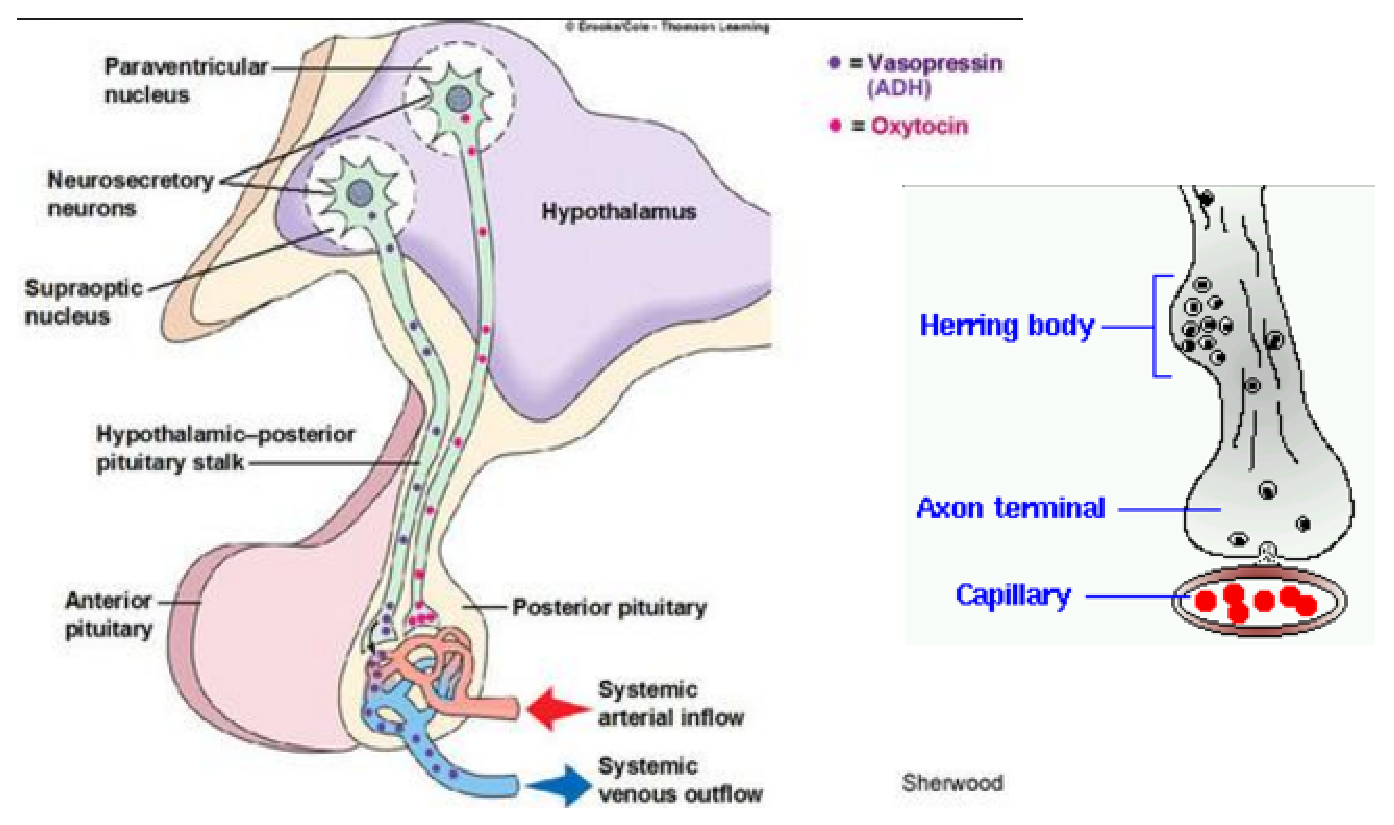
\includegraphics[height=4cm]{./images/posterior-pituitary-gland.eps}}
\caption{Magnocellular neurosecretory
cells from the two nuclei (paraventricular nucleus, supraoptic
nucleus) in the hypothalamus with axonal
projections to the posterior pituitary
gland (Sect.\ref{sec:posterior-pituitary-gland}). The hormones are stored in
the swelling region in the axons called Hering
body, before it can be released into the
blood stream at the posterior pituitary
gland}\label{fig:posterior-pituitary-gland}
\end{figure} 


{\bf Magnocellular neurosecretory cells} (MNCs) are very large cells, and
are most extensively studied in rat. They generally have a long axon
with about 10,000 neurosecretory terminals and many axon swellings
that store very large numbers of hormone-containing vesicles. 

Cells can be activated by stressful and/or physiological changes Upon activated,
the posterior pituitary gland release hormone-containing vesicles into the blood
stream. These vesicles are released from the axon swellings and nerve terminals
by {\it exocytosis} in response to calcium entry through voltage-gated channels.

The cells have two to three long dendrites which receive about 10,000
synapses from afferent neurons. 


\subsection{Mitral cells}
\label{sec:mitral-cell}

Mitral cells together with tufted cells form the two principal neurons in
olfactory bulb and provide an {\it obligatory relay} for all olfactory
information entering from the olfactory nerve. The relayed signal is then
projected to a number of brain areas, including piriform cortex, entorhinal
cortex, and amygdala.


Mitral cells receive information from the axons of at least four cell types:
olfactory sensory neurons, periglomerular neurons, external tufted cells and
granule cells.
\begin{itemize}

  \item excitatory inputs: 
  
  \begin{enumerate}
    \item  olfactory receptor neurons  (Sect.\ref{sec:olfactory-nerve}),
    forming synapses in neuropils called glomeruli.

    \item external tufted cells on their primary dendrites. 
  \end{enumerate}
 
  \item inhibitory inputs: arises either from granule cells onto their lateral
  dendrites and soma or from periglomerular cells onto their dendritic tuft.
\end{itemize}


In terms of organization, mitral cells are distinguished by the position of
their somata located in an orderly row in the mitral cell layer of the bulb.
They typically have a single primary dendrite, which they project into a single
glomerulus in the glomerular layer, and a few lateral dendrites that project
laterally in the external plexiform layer.
 
Mitral cells send their axons by way of the lateral olfactory tract (LOT) to
ipsilateral cortical structures.
 
 
However, the mechanism of how the input is encoded is still a big debate. The
odor responsiveness of the 20-40 mitral cells connected to a single glomerulus
(called sister mitral cells).




\subsection{Microneurons}
\label{sec:microneurons}

{\bf Microneurons} are found in the isothalamus (Sect.\ref{sec:thalamus}).
They have short and thin dendrites and short axon(s) and thus belong to local
circuitry neurons. As TC are also found in the isothalamus, their percentage in
comparison to thalamocortical neurons varies across species, highly increasing
with evolution.

Microneuron's neurotransmitter is GABA. The dendrites receive the input only
from pyramidal neurons in the cortex; while their axons contact thalamocortical
or other local circuitry neurons.
The connection back to the thalamocortical neurons create "triads" modulating
the thalamocortical output.

\subsection{Neuroendocrine cells}
\label{sec:neuroendocrine-cell}

Neuroendocrine cells are cells that receive neuronal input (neurotransmitters
released by nerve cells or neurosecretory cells) and, as a consequence of this
input, release message molecules (hormones) to the blood.
They  bring about an integration between the nervous system and the endocrine
system (Chap.\ref{chap:Endocrine-System}), a process known as neuroendocrine
integration.

Example:
\begin{enumerate}
  \item  cell of the adrenal medulla (innermost part of the adrenal gland),
  which releases adrenaline to the blood - Sect.\ref{sec:adrenal-medulla}. 
  
  The adrenal medullary cells are controlled by the sympathetic division of the
  autonomic nervous system. 
  
  \item 
\end{enumerate}

\subsection{Neuroglia cell}
\label{sec:neuroglia-cell}

Neuroglia cells are found in cerebellum (Sect.\ref{sec:cerebellum}).



\subsection{Noradrenergic neurons}
\label{sec:noradrenergic-neurons}

{\bf Noradrenergic neurons} refers to neurons that release neurotransmitter
norepinephrine (Sect.\ref{sec:norepinephrine}).

The largest group of NE neurons is the A6 group or locus coeruleus (LC), which
supplies NE to the majority of forebrain structures.

{\it NOTE: For A8-A16 cells, check Sect.\ref{sec:dopaminegic_neurons}}
\begin{enumerate}
  \item A1 cells = the group of noradrenergic neurons found in the vicinity of
  lateral reticular nucleus of the medullary reticular formation
  (Sect.\ref{sec:reticular-formation})
  
  \item A2 cells = 
  
  \item A3 cells = 
  \item A4 cells = 
  \item A5 cells = 
  \item A6 cells = 
  \item A7 cells =
  \item A6sc cells = 
  \item Acg cells =    
\end{enumerate}

{\it NOTE: For C1-C16 cells, check Sect.\ref{sec:dopaminegic_neurons}}



\subsection{Non-spiking neurons}
\label{sec:non-spiking-neurons}


\subsection{Orexin neuron}
\label{sec:orexin-neuron}

{\bf Orexin neuron} (or orexin-producing neuron) represent a small population of
neurons found in lateral and posterior hypothalamus. There are about 70,000 of
them in human brain. These neurons project from the lateral hypothalamus to
neurons and brain regions that modulate wakefulness.
However, the axons from these neurons extend throughout the entire brain and
spinal cord, where there are also receptors for orexin. 

Orexin (Greek: orexis, meaning "appetite"), also called hypocretin, is an {\bf
excitatory neuropeptide} that regulates arousal, wakefulness, and appetite,
which was discovered by two groups in 1998.
NOTE: hypocretin is used to refer to the genetic products and orexin is used to
refer to the protein products.

There are 2 types of orexin:  orexin-A and -B (hypocretin-1 and -2). 
\begin{enumerate}
  \item  Orexin-A is 33 amino acid residues long
  
  \item  orexin-B is a linear 28 amino acid
\end{enumerate}
The receptors bound to orexin are two G-protein coupled orexin receptors, OX1
and OX2




\subsection{Olfactory neurons}
\label{sec:olfactory-nerve}

The specialized olfactory receptor neurons are located in the olfactory mucosa
of the upper parts of the nasal cavity.
Olfactory receptor neurons continue to be born throughout life and extend new
axons to the olfactory bulb (Sect.\ref{sec:olfactory-bulb}) where it forms the
synapse with mitral cells (Sect.\ref{sec:mitral-cell}).

The sense of smell (olfaction) arises from the stimulation of olfactory (or
odorant) receptors by small molecules of different spatial, chemical, and
electrical properties that pass over the nasal epithelium in the nasal cavity
during inhalation.

\url{http://en.wikipedia.org/wiki/Olfactory_nerve}

\subsection{-- dopaminergic periglomerular neurons (DA-PG cells)}
\label{sec:olfactory-nerve-dopaminergic-periglomerular-neuron}
\label{sec:periglomerular-cell}
\label{sec:DA-PG-cells}

Dopaminergic (DA) periglomerular (PG) neurons are critically placed at the entry
of the bulbar circuitry (Sect.\ref{sec:olfactory-bulb}), directly in contact
with both the terminals of olfactory sensory neurons and the apical dendrites of projection neurons.

Dopaminergic (DA) neurons represent an estimated 10 - 16\% of the neurons residing
in the most external (glomerular) layer of the main olfactory bulb (MOB) (Halasz
et al., 1977; McLean and Shipley, 1988) - Sect.\ref{sec:glomerulus}.


Dopaminergic perglomerular neurons are autorhythmic and are the target of
numerous terminals releasing a variety of neurotransmitters.


IKir could be distinguished from the hyperpolarization-activated current (Ih) by
showing full activation in <10 ms, no inactivation, suppression by Ba2+ in a
typical voltage-dependent manner (IC50 208 $\muM$) and reversal potential nearly
coincident with EK.  
\begin{itemize}
  \item  Ba2+ (2 mM) induces a large depolarization of DA-PG cells, paralleled
  by an increase of the input resistance, leading to a block of the spontaneous activity
  
  \item The Kir current is negatively modulated by intracellular cAMP
  
Reduction in its amplitude is induced by forskolin or 8Br-cAMP

  
\end{itemize}

\subsection{Pallidal neurons (globus pallidus neuron, GP neuron)}
\label{sec:Pallidal-neurons}
\label{sec:GP_neurons}
\label{sec:globus-pallidus_neurons}

Pallidal neurons are neurons in the Globus pallidus
(Sect.\ref{sec:globus_pallidus}) and they are inhibitory neurons
(Sect.\ref{sec:inhibitory-cell}).

\subsection{Parvalbumin-positive interneuron (PV-positive, PV+)}
\label{sec:parvalbumin-positive-interneuron}
\label{sec:PV+-neuron}
\label{sec:PV-positive-neuron}

Parvalbumin-positive interneurons (PV-positive, PV+) are inhibitory interneuron
(Sect.\ref{sec:interneurons}), i.e. releasing GABA, and express paravalbumin
(Sect.\ref{sec:parvalbumin}). It uses GAT-1 for GABA reuptake
(Sect.\ref{sec:GAT-1}).

PV-positive interneurons is found in 
\begin{enumerate}
  \item reticular thalamus, 
  
  \item expressed predominantly by chandelier and basket cells in the cortex.

PV+ interneurons are subdivided into basket, axo-axonic, bistratified, and
oriens-lacunosum moleculare (O-LM) cells, each targetting a different types of
pyramidal neurons.

  
  \item in Purkinje cells (Sect.\ref{sec:Purkinjie_nerves}) and molecular layer
  interneurons of cerebellum
  
  \item 
\end{enumerate}

They are also thought to give rise to gamma waves recorded in EEG
(Sect.\ref{sec:gamma-wave}).

\subsection{somatostatin-positive interneuron (STT-positive, STT+)}
\label{sec:somatostatin-positive-interneuron}
\label{sec:STT-positive-interneuron}

\subsection{rose-hip interneurons (specific to human only)}

Inhibitory neurons are considered to act like the brakes in a car. They tell
other brain cells when to slow down.

Members of Hungarian neuroscientist Gabor Tamas's lab were recording electrical
signals from inhibitory neurons taken from the cortex of two men who had died
(Boldog et al., 2018).
\url{https://www.nature.com/articles/s41593-018-0205-2}

"In the course of doing these recordings, he started to notice a very
distinctive type of cell that, to him, had the shape of a rose after the petals
have fallen off, so he called them 'rose hip cells'.
By chance, scientists at the Allen Institute had also identified these cells
using an entirely different approach, a new technique that allowed them to
detect the genes that are switched on in human brain cells.
So the researchers combined what they had learned and confirmed that rose hip
cells were a distinct subtype of inhibitory neurons.

These cells are supprisingly found to be only in humans.
The brain cells have been named "rose hip neurons" by a team at the University
of Szeged in Hungary, which played a key role in the discovery.
\begin{enumerate}
  \item  10 GABAergic interneuron subtypes with combinatorial gene signatures
  in human cortical layer 1 
  
  \item make homotypic gap junctions, predominantly target apical dendritic
  shafts of layer 3 pyramidal neurons,  and inhibit backpropagating pyramidal
  action potentials in microdomains of the dendritic tuft
  
  \item and characterize a group of human interneurons with
  anatomical features never described in rodents, having large ‘rosehip’-like
  axonal boutons and compact arborization
  
  \item These rosehip cells show an immunohistochemical profile (GAD1+CCK+,
  CNR1–SST–CALB2–PVALB–) matching a single transcriptomically defined cell type
  whose specific molecular marker signature is not seen in mouse cortex. 
  
  
\end{enumerate}

The finding challenges earlier evidence that the human brain is merely bigger
and more sophisticated than a mouse brain. At some point, humans acquired at
least one kind of brain cell that a mouse doesn't have.

It is still possible that these newly identified neurons will also be found the
brains of primates like monkeys or chimps, Ed Lein of the Allen Institute for
Brain Science in Seattle says.

\textcolor{red}{FUNCTIONS}: 
Scientists aren't sure exactly what rose hip cells do, though they appear to be
involved in the controlling the flow of information in specific areas of the
brain.
\begin{enumerate}
  \item   potent local control of distal dendritic computation in cortical
  pyramidal neurons.
\end{enumerate}

\textcolor{red}{IMPORTANCE OF THE FINDING}:  "it throws some doubt on the
ability to use the mouse to study certain elements of human function and
disease," Lein says. And because rose hip neurons are a type of inhibitory
neuron, they could play a role in mental illness, he says.  If rosehip cells are
involved in brain disorders, it could help explain why so many brain drugs that
work in mice don't work in people
\url{https://www.npr.org/sections/health-shots/2018/08/27/642255886/a-new-discovery-may-explain-what-makes-the-human-brain-unique}


\subsection{projection neurons}
\label{sec:projection-neurons}

Broadly defined, projection neurons are neurons whose axons extend from the
neuronal cell body within the central nervous system (CNS) to one or more
distant regions of the CNS. Such neurons are likely to be essential to neuronal
integration for all sensory, associative and motor systems.

Modulatory projection neurons are the subclass of these neurons which have
modulatory (generally synonymous with metabotropic) actions on their target
neurons usually in addition to having classical (i.e., ionotropic) actions.

Example of projection neurons
\begin{enumerate}
  \item Sect.\ref{sec:pyramidal-neuron-neocortex}
\end{enumerate}

\subsection{Purkinje nerve cells}
\label{sec:Purkinjie_nerves}
\label{sec:mossy-fiber}
\label{sec:climbing-fiber}

Purkinje neurons are multi-polar neurons (Sect.\ref{sec:multi-polar-neurons})
and belong to a class of GABAergic neurons (Sect.\ref{sec:GABAergic-neurons})
located in the cerebellum (Sect.\ref{sec:cerebellum}). Based on the 4 zones in
the cerebellum (Sect.\ref{sec:cerebellum_zones}), Purkinje cells in different
zones project to different deep cerebellar nuclei.
Purkinje cells are riched with parvalbumin (PV), i.e. PC-positive neurons
(Sect.\ref{sec:PV+-neuron}).

The dendrites of each Purkinje cell have a very distinctive pattern (i.e.
fan-shaped) in that their branches all lie in one plane in which they assume the
shape of a fan (Ito, 1989).
The fan-shaped dendrites of adjacent cells lie parallel to each other.

The dendritic branches of each Purkinje cell receive excitatory synapses from
the branch terminations of a single afferent climbing fibre (CF); and also from
parallel fibers (PF).  The cerebellum ensures smooth and well-timed execution of
ongoing motor tasks, by making use of mainly two input sources
\begin{enumerate}
  \item climbing fibers (CF): carrying information about sensory events,
e.g. a touch sensation on a specific part of the skin.
  
  
  The climbing fibre is the axon of a neuron in the
  inferior olive (Sect.\ref{sec:inferior-olive-nucleus}), a nucleus in the medulla oblongata.

  
  \item mossy fibes (MF):  carrying information from many
  brain regions and thought to provide contextual information e.g.
regarding sensory input from different modalities as well as ongoing motor
activity and proprioceptive information.

MF signals are 'recoded' by the numerous cerebellar granule cells, which in
turn give rise to the so-called parallel fibers (PF).

\end{enumerate}
In the cerebellar cortex, the PFs and CFs converge on Purkinje cells (PC).
\textcolor{red}{A PC receives a plethora of PF inputs}, which modulate the PC's
intrinsic rapid spiking behavior, \textcolor{red}{and only one CF input}.
Likewise, each Purkinje cell receives over 100,000q synapses from 100,000
different parallel fibres (Konnerth et al., 1992).


Two striking features of Purkinje neurons {\it in vivo} are 
\begin{enumerate}
  \item regular, spontaneous firing (Bell and Grimm, 1969; Latham and Paul,
  1971) - spontaneous AP (Sect.\ref{sec:AP-neuron}) in the
absence of synaptic drive.

Thereby the neurons can exert a tonic, yet plastic, input to their target cells
in the deep cerebellar nuclei. The neuron expresses two ionic currents with
biophysical properties that are specialized for high-frequency firing: resurgent
sodium currents (Sect.\ref{sec:resurgent-sodium-current}) and potassium currents
mediated by Kv3.3 (Sect.\ref{sec:Kv3-channels}).

Llinas and Sugimori (1980a,b) attributed the distinctive firing properties of
Purkinje neurons to a variety of intrinsic membrane conductances in the neurons,
including voltage-activated calcium conductances and a persistent sodium
conductance. They suggested that this noninactivating sodium conductance is
located in the cell body of Purkinje neurons.

  \item upon stimulation of climbing fibers, formation of "complex spikes"
  consisting of multiple peaks (Eccles et al., 1966,1967; Martinez et al., 1971).
  
\end{enumerate}




\subsection{Pyramidal neurons}
\label{sec:pyramidal-neurons}
% \subsection{Projection neurons}

Pyramidal neurons (projection neurons) are multipolar neurons
(Sect.\ref{sec:multi-polar-neurons}) with a cell body shaped like a pyramid
(i.e. pyramidal profile or triangular-shaped somata), in
Fig.~\ref{fig:pyramidal}. Each pyramidal cell has a single axon and two distinct
dendritic trees:
basal dendrites (a few) and apical dendrite (only one). Apical dendrite is
longer, and often thicker than the other dendrites.
This is different from non-pyramidal neurons, e.g. interneurons -
Sect.\ref{sec:interneurons-cortical}.

Both axon and dendrites branch extensively so that a single pyramidal neuron can
communicate with thousands of others. Pyramidal neurons play important roles in
signaling control in the brain. Pyramidal neurons thus can receive input from axons
within its somatic vicinity and from axons of the cortical surface reaching
the apical dendritic tree.


\begin{figure}[hbt]
  \centerline{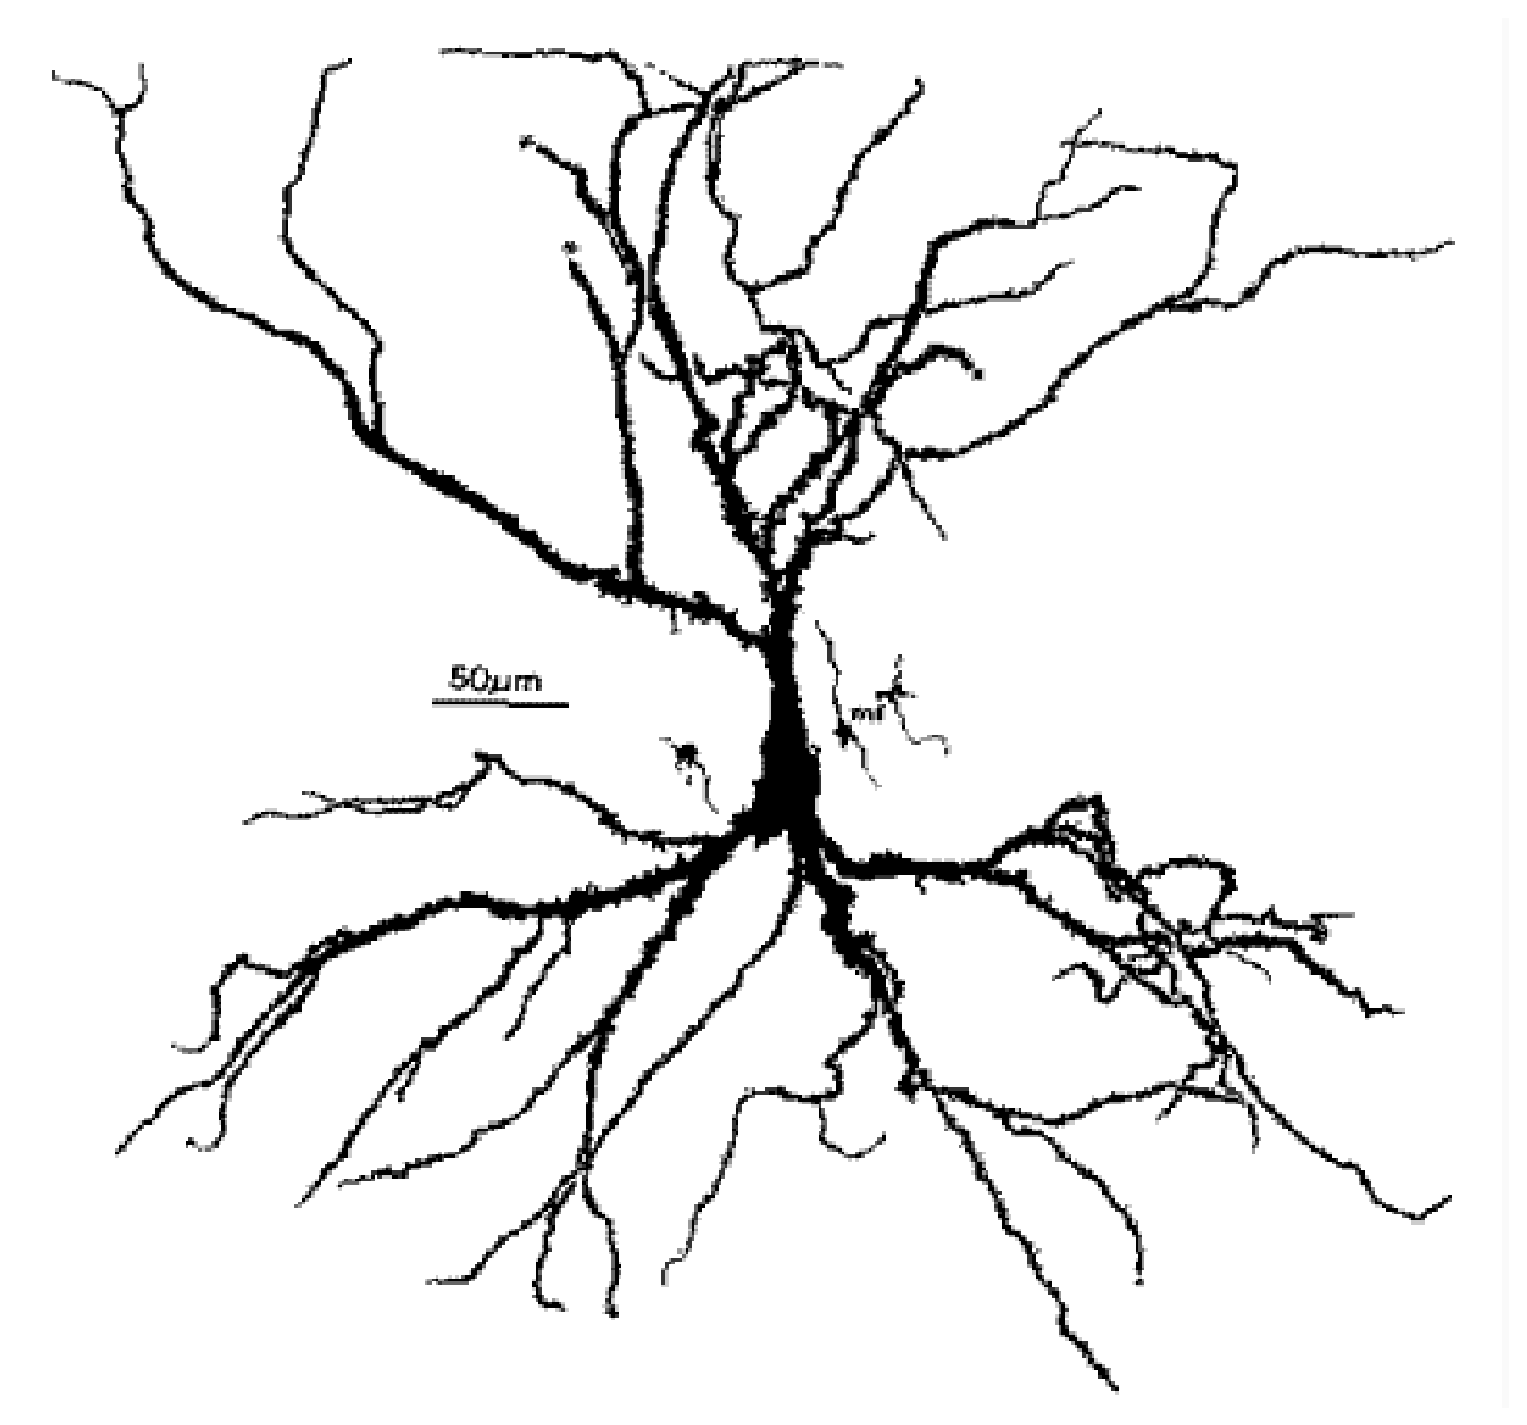
\includegraphics[height=5cm,
    angle=0]{./images/pyramidal_cell.eps},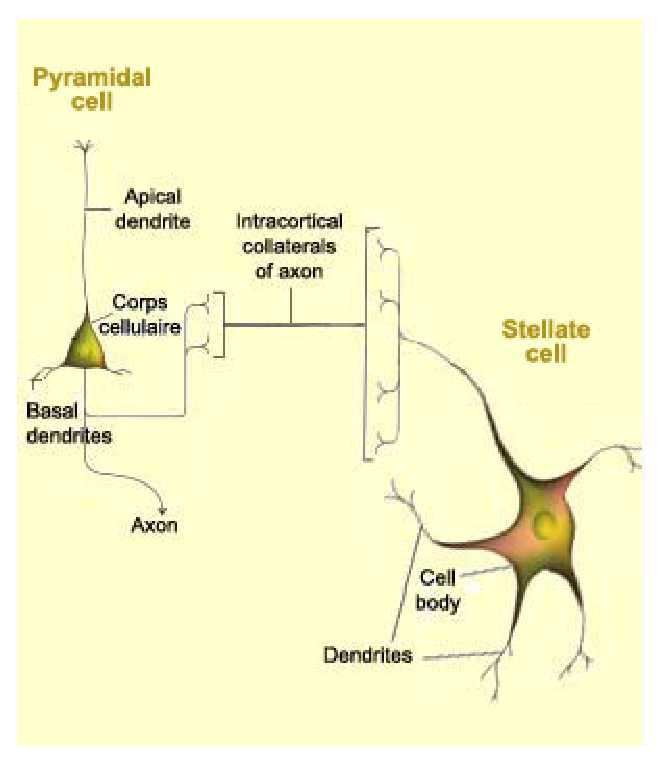
\includegraphics[height=5cm,
    angle=0]{./images/pyramidal_cell_02.eps}}
\caption{Pyramidal cell}
\label{fig:pyramidal}
\end{figure}

Pyramidal neurons are different not only at different regions of the brain
(e.g. neocortex vs. hippocampus), but also within a region, e.g. layer 2/3 vs.
layer 5 of neocortex.
\begin{enumerate}
  \item neocortex (Sect.\ref{sec:neocortex})
  \begin{itemize}
  \item Layer 2/3 pyramidal neuron (Sect.\ref{sec:pyramidal-neuron-layer-2/3})
  
  \item Layer 5 pyramidla neuron (Sect.\ref{sec:pyramidal-neuron-layer-V}) 

  \end{itemize}

 \item hippocampus (Sect.\ref{sec:hippocampus})
 \begin{itemize}
  \item CA3 pyramidal neuron
  
  \item CA1 pyramidal neuron
  
  \item subiculum pyramidal neuron - Sect.\ref{sec:subiculum}
 \end{itemize}  
\end{enumerate}
With unique morphological features, express different complements of
transcription factors, they ultimately serve different functions.


The dendritic membrane of pyramidal neurons contains active conductances: $\Na$,
$\K$ and $\Ca$ channels. 
\begin{itemize}
  \item Studies of proximal stimulation: 

During subthreshold synaptic stimulation
mostly in the proximal parts of apical dendrites, it can activates voltage-dependent $\Ca$ and
$\Na$ channels (Markram \& Sakmann, 1994; Magee \& Johnston, 1995; Magee,
Christofi, Miyakawa, Christie, Lasser-Ross \& Johnston, 1995). 

  \item Studies of distal stimulation (tuft dendrites at distant $> 600\mum$
  from soma):
  
  The contribution of active dendritic conductances to the amplitude and time
  course of EPSPs in the distal dendrites of the apical tuft is of particular
  interest. The data showed that such distal stimulation can initiate $\Ca$
  spikes, which remained locally restricted to the distal dendrites and evoke a
  local dendritic [Ca2+]i transient \citep{schiller1997}.
  
\end{itemize}




\subsection{-- pyramidal neurons in cortex}
\label{sec:pyramidal-neuron-neocortex}

In mammalian, pyramidal neurons are the most numerous excitable units in the
cerebral cortex (Sect.\ref{sec:cerebral_cortex}), specifically at the frontal
lobe (Sect.\ref{sec:frontal-lobe}) - (Sect.\ref{sec:cortical-neurons}). It is
also found in {\it hippocampus} (Sect.\ref{sec:hippocampus}) and {\it amygdala}
(Sect.\ref{sec:amygdala}).
Besides mammalian, pyramidal neurons are also found in birds, fish and reptiles,
yet not found in amphibians~\cite{nieuwenhuys1994}.

Within the mature neocortex, distinct populations of projection neurons are
located in different cortical layers (Sect.\ref{sec:neocortex-6-layers}) and
areas (Sect.\ref{sec:neocortex_functional-column}).

In cortex, pyramidal neurons (particularly layers 5, 6) are the only neurons
that send signals out of their local region to other parts of the brain,
example: Sect.\ref{sec:subiculum}. For this reason, layer 5 or 6 pyramidal
neurons are also called {\bf projection neurons}
(Sect.\ref{sec:projection-neurons}) - a class of cortical neurons
that extend axons projecting to (1) distant
intracortical, (2) subcortical and (3) subcerebral targets.
\textcolor{green}{The majority in number of pyramidal cells in the
  regions associated with advanced cognitive functions suggests the
  understanding of these neurons is necessary to elucidate the neural
  bases of such functions.}

  

\begin{figure}[hbt]
  \centerline{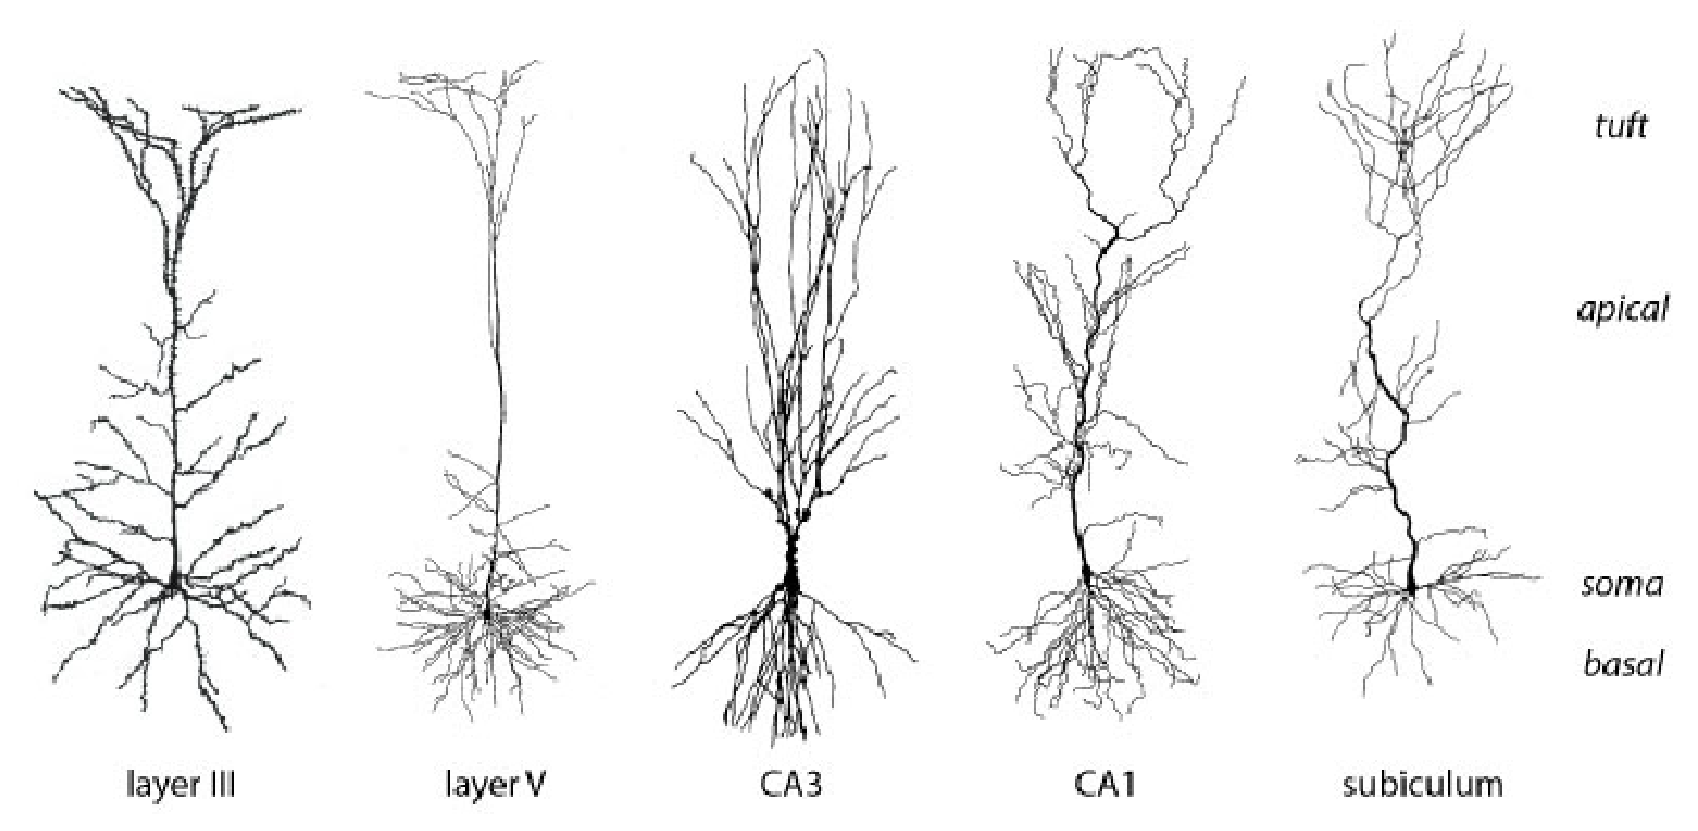
\includegraphics[height=7cm,
    angle=0]{./images/pyramidal_classes.eps}}
\caption{Different classes of pyramidal neurons}
\label{fig:pyrmidal_class}
\end{figure}

Despite the sterotypical in structure, pyramidal neurons in the neocortex are
still classified into different types, depending upon their locations in the
brain, as shown in Fig.~\ref{fig:pyrmidal_class} \citep{spruston2008}:
\footnote{\url{http://www.scholarpedia.org/article/Pyramidal_neuron}}:
\begin{itemize}
  \item layer II of cortex: Sect.\ref{sec:pyramidal-neuron-layer-II}

  \item layer III of cortex: Sect.\ref{sec:pyramidal-neuron-layer-III}
  

  \item layer V of cortex: a very long apical dendrite that span
  the entire cortical column, thus receiving input from all six layers. 
  
  Betz cells are giant pyramidal cells located at the layer V of the grey
  matter, first discovered by the scientist Betz in 1874. They are the largest
  neurons in the CNS, sometimes reaching 10$\mum$ in diameter.  
  
  The pyramidal cells in layer V are classified into 2 main classes (5a and 5b)
  that differ in dendritic morphologies, electrical properties, axonal
  projection, and the thalamocortical input they receive.

  \begin{enumerate}
    
    \item Layer Vb pyramidal cells (L5b PCs, thick-tufted layer V pyramidal
    (TTL5) neuron) - on the deeper part of layer V:
    Sect.\ref{sec:pyramidal-neuron-layer-Vb}
    
    \item Layer Va pyramidal cells (L5a PCs) - on the superficial part of layer
    V:   Sect.\ref{sec:pyramidal-neuron-layer-Va}
  \end{enumerate}

\end{itemize}
These names already tell the location where the pyramidal neurons of that type
reside.

Among the different types of cortical projection neurons, {\it subcerebral
projection neurons} are widely studied, which is found in layer Vb of the
neocortex. It extends a primary axon through the internal capsule, cerebral
peduncle and pyramidal tract towards the spinal cord. The most well-studied
subtype of subcerebral projection neuron is the {\bf corticospinal motor
neurons} (CSMNs) - Sect.\ref{sec:CSMN}.


\begin{figure}[hbt]
  \centerline{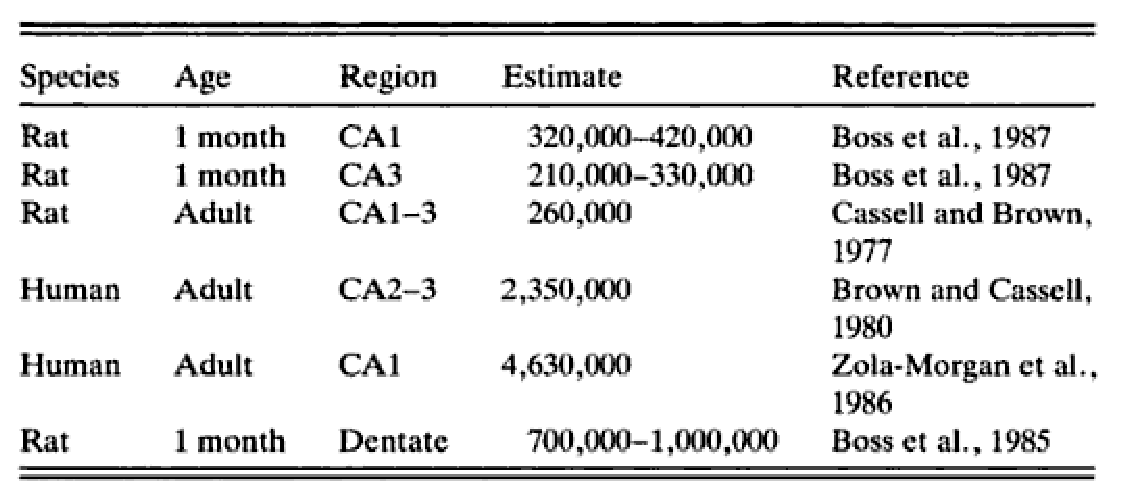
\includegraphics[height=5cm,
    angle=0]{./images/hippocampus_number.eps}}
 \caption{Estimate the number of pyramidal or granule cells in
   hippocampus}
\label{fig:pyramidal_number}
\end{figure}



\subsection{ * Pyramidal neuron: Layer II}
\label{sec:pyramidal-neuron-layer-II}

Layer II pyramidal neurons are smaller than that in Layer III.
Most of Layer II pyramidal neurons have their somata in the deepest third of the
layer. 
\begin{itemize}
  \item triangular somata
  \item a thick apical dendrites extending into layer I
  \item a thinner basal dendrites extending into layer III
\end{itemize}
Both apical and basal dendrites branch extensively and studded with spines with
an even higher density than in layer II stelate cells (Klink and Alonso, 1997).

\subsection{ * Pyramidal neuron: Layer III}
\label{sec:pyramidal-neuron-layer-III}

Layer III pyramidal neurons in different regions of the cortex: first (V1),
second (V2), dorsolateral (DL) and fundus of the superior temporal (FST) areas
in marmoset monkey visual cortex.
\begin{enumerate}
  \item V1, V2 areas: early stages of visual processing

  \item DL: specialized in analysis of shape
  \item FST: specialized in analysis of motion
\end{enumerate}

\begin{verbatim}
                         mean basal            
                         dendritic area
                         (um^2)
V1 pyramidal neurons     1.84e4 
V2 ...                   2.32e4
              (i.e. 1.26 x larger thanV1)
DL ...                   2.75e4
              (i.e. 1.5 x larger thanV1)
FST ...                  4.26e4
              (i.e. 2.3 x larger thanV1)

\end{verbatim}
The increase in basal dendritic field area of layer III pyramidal cells may
be explained to allow more extensive sampling inputs as required by higher-order
processing of visual information (Elston et al., 1996).


\subsection{* Layer 2/3}
\label{sec:pyramidal-neuron-layer-2/3}

Most of the time, Layer II and Layer III neurons are treated as the same, under
the name Layer 2/3 pyramidal neurons. Layer 2/3 (L2/3) pyramidal neurons are the
most abundant cells of the neocortex.

Despite their key position in the cortical microcircuit, synaptic integration in
dendrites of L2/3 neurons is far less understood than in L5 pyramidal cell
dendrites, mainly because of the difficulties in obtaining electrical recordings
from thin dendrites.

INPUT:
\begin{enumerate}
  \item predominantly from other L2/3 pyramidal neurons and L4 spiny stellate
  neurons (Lubke et al., 2003; Binzegger et al., 2004).

These inputs project almost exclusively to the basal and apical oblique
dendrites

  \item feedback connections from higher cortical areas and nonspecific thalamic
  nuclei (Felleman and Van Essen, 1991).
  
These inputs are thought projecting to apical tuft.
\end{enumerate}

Unlike L5 cells, L2/3 dendrites displayed little sag in response to long current
pulses, which suggests a \textcolor{red}{low density of Ih in the dendrites and
soma}.  This was also consistent with a slight increase in input resistance
(Sect.\ref{sec:input-resistance}) with distance from the soma. Lakurm et al.
(2007) reported for the first time the simultaneous recording of somata and
apical dendrites, in brain slices of rat somatosensory cortex.

\begin{itemize}
  
  \item  Brief current injections into the apical dendrite evoked relatively
  short (half-width 2-4 ms) dendritic spikes that were isolated from the soma
  for near-threshold currents at sites beyond the middle of the apical dendrite.
  
  \item Trains of somatic action potentials (APs) above a critical frequency
  (130 Hz), which was slightly higher than in L5 neurons, 
  can create regenerative dendritic potentials and large concomitant calcium
  transients.
  
  \item backpropagating  somatic APs can facilitate the initiation of dendritic
  spikes; which subsequently could cause an additional AP at the soma.
  
  apical dendrites of L2/3 neurons sustain active backpropagation of action
  potentials supported by dendritic Na+ channels (Waters et al., 2003; Waters
  and Helmchen, 2004) and have a concomitant influx of calcium ions (Svoboda et
  al., 1999).
  
  \item  (similar to L5 neuron) distal dendritic calcium transients are
  sensitive to a long-lasting block by GABAergic inhibition
\end{itemize}

It is believed that L2/3 pyramidal neurons can generate dendritic spikes,
sharing with L5 pyramidal neurons fundamental properties of dendritic
excitability and control by inhibition (Larkum et al., 2007).


\subsection{ * Pyramidal neuron: Layer V}
\label{sec:pyramidal-neuron-layer-V}

Layer V Pyradimal neurons of neocortex are classified into 2 groups; which are
different in dendritic morphology, thalamocortical input they receive, and
location of the soma within layer V.

\begin{itemize}
  \item Layer Va
  
  \item Layer Vb
\end{itemize}

Layer V pyramidal neurons:
\begin{itemize}
  \item local dendrites extending from its base (i.e. {\bf basal dendrites}
  branching out profusely in all directions) for receiving local communication,

   \item a long {\bf apical dendrite} extending from the pyramid's apex toward
   the cortical surface for receiving signals from Layer 2/3 neurons
   (Sect.\ref{sec:layer-II}).
   
  \item axons: there are two types of axons in the pyramidal cells. The axon of
  the pyramidal neuron (1) grows numerous branches in the vicinity of the cell
  body; (2) the main axon projecting to the subcortical areas and some
  continue into the white matter and leave the cortex there.

\textcolor{red}{It is believed that both local and remote synapses of these
axons of the pyramidal neurons are excitatory}. Pyramidal neurons are
glutamatergic neurons (Sect.\ref{sec:glutamatergic_neurons}).

\end{itemize}


In L5 neurons, distal inputs can induce AP bursts via dendritic Ca2+ spikes

\subsection{- * Pyramidal neuron: Layer Va}
\label{sec:pyramidal-neuron-layer-Va}

Thin-tufted neuron, project to other parts of the cortex, and they tend to
discharge  spikes with no adaptation (Sect.\ref{sec:tonic-spike})
    
    
\subsection{ -* Pyramidal neuron: Layer Vb}
\label{sec:pyramidal-neuron-layer-Vb}

Layer Vb neurons have a thick-tufted dendrite (i.e. large diameter of apical
dendrites) extending its dendritic tree to all six layers of the mammalian
neocortex and projects its axons to subcortical targets (tectum, brainstem, and
spinal cord).

Layer Vb Pyramidal neurons tend to discharge a short burst of spikes in the
beginning of a spike train (Sect.\ref{sec:mixed-mode}).

The key active properties of L5b PCs involve two main spiking zones
\begin{itemize}
  \item $\Na$ action potential initiated at the perisomatic region
      
  \item second spiking zone at distal apical dendrites: $\Ca$ spikes are
  generatd in response to intensive stimulation from dendrite and soma (in
  vitro).
\end{itemize}

BAP-activated $\Ca$ spikes (BAC) mechanism: In vitro studies have demonstrated
that the two spiking zones interact with each other, whereby the coincidence of
the back-propagating action potential (BAP) from the first zone and local
excitatory postsynaptic potential (EPSP) at the distal dendrites triggers a
dendritic $\Ca$ spike, which in turns which in turn triggers one or more
additional perisomatic Na+ APs.



\subsection{-- pyramidal neurons in hippocampus}
\label{sec:pyramidal-neuron-hippocampus}

Place cells (Sect.\ref{sec:place_cells}) is a type of pyramidal neurons in the
hippocampus.

Pyramidal cells + granule cells (Sect.\ref{sec:granule_cells}) = can produce
excitation with fast (millisecond). Pyramidal cells are the dominant in
hippocampus. Granule cells, with a lower amount, mainly in dentate
gyrus (Sect.\ref{sec:granule_cells}).

In hippocampus, the major difference between CA1 and CA3 pyrimidal cells is that
the latter have a much greater tendency to burst spontaneously or following
brief intracellular current pulses~\cite{wong1981agh}. In rats, they can fire
brief bursts    of 2-10 action    potentials    at frequencies     of 100-300 Hz
(i.e. complex spikes) during which    spikes typically become     
broader towards the end of  the burst.
  \begin{enumerate}  
  \item CA3 of hippocampus:

The number of cells in rat CA3 region {\it in vivo} is of an order of
magnitude larger than the number in the largest {\it in vitro} guinea
pig preparation. In a longitudinal CA3 slice ($400\mu$ thick and 10mm
long), it has 20,000 pyramidal cells. CA3 region of a transverse slice
may contain 3,000-5,000 cells.
  
  \item CA1 of hippocampus:
  \end{enumerate}
  

The input to pyramidal neurons in hippocampus:
\begin{itemize}
  \item inhibitory effect from basket cells (Sect.\ref{sec:basket-cell-hippocampus})
  at its somata and proximal dendrites.
  
\end{itemize}

Currents:
\begin{enumerate}
  \item BK-like $\Ca$-dependent $\K$ current:
  \begin{itemize}
    \item initially described as a sustained current $I_c$ (Lancaster \& Adams,
    1986).

    \item some voltage-clamp and single-channel studies also reported evidence
    for a fast transient, tetraethylammonium (TEA)-sensitive Ca-dependent K+
    current - $I_\text{CT}$ in CA3 (Zbicz \& Weight, 1985) and
    CA1 pyramidal cells (Storm, 1987c, 1990; McLarnon, 1995; Hicks \& Marrion,
    1998). 
    
    It is reminiscent of fast inactivating BKchannel current found in adrenal
    chromaffin cells (Solaro \& Lingle, 1992; Lingle et al. 1996) -
    Sect.\ref{sec:BK(Ca)-type-I}.
    
  \end{itemize}
  
  
\end{enumerate}
    
\subsection{ * Place cells}
\label{sec:place_cells}

The brain store information about the spatial environment that the animal has
traveled before.

{\bf Place cells}: is a type of pyramidal neurons
(Sect.\ref{sec:pyramidal-neurons}) in the hippocampus that becomes active when
the animal enters a particular place in the environment. These cells enable a
sense of place and navigation (analogous to {\it receptive field} in sensory
neurons - Sect.\ref{sec:receptive-field}).

\url{https://knowingneurons.files.wordpress.com/2013/04/place-cell-animation.gif?w=1000&h=607,}
The animation suggested the place fields are defined with respect to the outside
world (allocentric), rather than the body (egocentric) \citep{moser2004}.
In other words, the brain somehow can create a cognitive map, and when it
recognizes a familar environment, place cells in the associated place field will
fire.
\url{http://hargreaves.swong.webfactional.com/place.htm}

Place cells forming a cognitive map  are first found
in rat by O'Keefe and Dostrovsky~\cite{keefe1971hsm}. Later, Ekstrom et
al.~\cite{ekstrom2003hsn} also found cells with similar properties in human
hippocampus. \textcolor{red}{In CA1 and CA3, place cells are believed to be
{\bf pyramidal cells}} (Sect.\ref{sec:hippocampus}), while those in dentate
gyrus (Sect.\ref{sec:dentate_gyrus}) are believed to be granule cells
(Sect.\ref{sec:granule_cells}). Dr. John O'Keefe, Dr. May-Britt Moser and Dr.
Edvard I. Moser shared the Nobel prize for this discovery in 2014
\url{http://www.nobelprize.org/nobel_prizes/medicine/laureates/2014/advanced-medicineprize2014.pdf}
 
Place field of new environment is established in the animal within minutes and
it tends to be stable over repeated exposures to the same environment.  When an
animal is in a specific environment, there is an increasing frequency of firing
in the cells of the corresponding place field, e.g. from virtually zero outside
the field to as much as 100 Hz in the middle of the place field.
In any particular environment, about 40-50\% of hippocampal place cells will be
active.  

Spatial learning is achieved via {\it synaptic plasticity}
(Sect.\ref{sec:synaptic_plasticity}), with NMDA glutmate receptor (NMDAR - for
controling synaptic plasticity and memory function) and AMPA glutamate receptor
(AMPAR) - Sect.\ref{sec:glutamate_receptor}. The form of neural plasticity known
as {\bf long-term plasticity} (Sect.\ref{sec:LTplasticity}) is believed to be
one of the main neural mechanism by which memory is stored in brain.

% {\bf NOTE}: Calcium flux through NMDAR is thought to play critical
% role in synaptic plasticity. Calcium enter postsynaptic dendritic spine via
% NMDAR only when presynaptic activation and postsynaptic depolarization
% occur at the same time. AMPAR mediate fast synaptic transmission in
% the CNS (Sect.\ref{sec:synaptic_transmission}).

\subsection{-- subiculum}

Subiculum: the pyramidal neurons in the subiculum exhibit transitions between
two modes of action potential output: bursting and single spiking
(Sectt.\ref{sec:subiculum}).
  
The transitions between these two modes is thought to be important for routing
information out of the hippocampus.


\subsection{Meynert cell}
\label{sec:Meynert-cell}

Meynert cells are indeed pyramidal cells located in the cerebral cortex near the
calcarine fissure (where primary visual cortex V1 is concentrated), and were
discovered by Theodore Meynert.

\subsection{Stellate cells}
\label{sec:stellate_cells}


{\bf Stellate cells} are neurons with several dendrites radiating from the cell
body giving them a star shape. From Sholl (1956), stellate cells are neurons
that receive the excitation only from axons that reach the vicinity of the cell
body. They are found mainly in Layer IV of cortex (Sect.\ref{sec:layer-IV}).

Stellate cells can be excitatory or inhibitory. The three most common stellate
cells
\begin{enumerate}

  \item excitatory spiny stellate interneurons (found in Layer IVc of V1 region
  in the visual cortex)

The excitatory stellate cells are often having dendrites with spines attached to
them, thus giving them the name {\bf spiny stellate cells}.
% Cortical spiny stellate cells are found in layer IVc of the V1 region in the
% visual cortex.
Cortical spiny stellate cells have a 'regular' firing pattern.
They receive excitatory synaptic fibres from the thalamus and process feed
forward excitation to 2/3 layer of V1 visual cortex to pyramidal cells.

  \item inhibitory aspiny stellate  interneurons.

Inhibitory stellate cells have very few spines on the dendrite, giving them the
name {\bf smooth stellate cells} (or sparsely spinous stellate cells)

  \item inhibitory interneurons (found in Layer I of the neocortex - Sect.\ref{sec:neocortex})

Cerebellar stellate cells synapse onto the dendritic arbors of Purkinje
cells
  


\end{enumerate}
\url{http://en.wikipedia.org/wiki/Stellate_cell}

\subsection{* inhibitory interneurons (layer I)}

See Sect.\ref{sec:stellate_cells}

\subsection{* excitatory spiny stellate interneuron (layer IVc of V1 region)}

See Sect.\ref{sec:stellate_cells}

\subsection{* inhibitory aspiny stellate interneuons}

See Sect.\ref{sec:stellate_cells}

\subsection{Serotonergic neurons}
\label{sec:serotonergic-neuron}


{\bf Serotonergic neurons} are neurons that release neurotransmitter serotonin
(Sect.\ref{sec:serotonin}).

Serotonergic neurons are found in 
\begin{enumerate}
  \item  the raphe nuclei (Sect.\ref{sec:raphe-nuclei}) of the reticular
  formation (Sect.\ref{sec:reticular-formation}); and these neurons play an important role
in regulating mood, appetite, and sleep. Serotonin also has some cognitive
functions, including memory and learning.

\end{enumerate}

These neurons have strong connnection to subgenual anterior cingulate -
Sect.\ref{sec:subgenual-cortical-area}.

Until today, the circuitry controlling serotonergic neurons remain
uncharacterized.

\subsection{Spiny neurons}
\label{sec:spiny-neurons}

Spiny neurons are projection neurons (Sect.\ref{sec:projection-neurons}) found
in the striatum. 

\subsection{Spinal motor neurons}
\label{sec:spinal-motor-neurons}

Spinal motor neurons are multi-polar neurons
(Sect.\ref{sec:multi-polar-neurons}) found in spinal cord
(Sect.\ref{sec:spinal_cord}).

\subsection{Thalamocortical neurons (TC) - thalamic relay neurons}
\label{sec:thalamocortical-neuron}
\label{sec:thalamic-relay-neuron}


All neocortical areas receive thalamic inputs, via the so-called {\bf
thalamocortical pathways}.
\begin{enumerate}
  \item first-order thalamic relay: 
  
  \item high-order thalamic relay
\end{enumerate}

Thalamic relay neurons are interneurons (Sect.\ref{sec:interneurons}), with
the capbility of multiple distinct firing modes, depending on the holding
level of stimulus.
\begin{enumerate}
  \item depolarized step $I_\app = 14 \mu A/\cm^2$: generate continuous spiking
  (CS) activity - {\bf relay mode}.
  
The relay mode corresponds to the transmission of sensory information through
the thalamus to the cortex in the awake state (Steriade et al. 1990).
  
  \item small depolarized step $I_\app = 8 \mu A/\cm^2$: show only passive
  response
  
  \item at the end of hyperpolarized step $I_\app = -3 \mu A/\cm^2$: generate a
  single rebound LTS burst upon the release of the hyperpolarized current.

Bursting is seen naturally during certain phases of sleep, when neuromodulators
lead to hyperpolarization in the thalamus, and during absence seizures (Coulter
et al. 1989b; Steriade et al. 1990).
  
MECHANISM: At hyperpolarized current, a transient calcium current (T-type)
slowly deinactivates and, on release from this voltage level, mediates a slow
depolarizing wave, the low-threshold spike (LTS). This rebound excitation
frequently exceeds the voltage threshold for the generation of sodium action
potentials so that a burst of spikes rides. 
   
   \item Other than on release, bursting behavior may
occur repetitively (1-10 Hz) for maintained hyperpolarizing
stimuli in an appropriate range 
\end{enumerate} 

Rodent thalamocortical relay cells have the interesting property of being able
to generate action potentials in either of two modes, both in vivo and in vitro:
\begin{itemize}
  \item single spike or tonic firing in which AP is generated one at a time in
  trains

Rate of single spike depends on the strength of depolarization. 

  \item burst firing in which the
  cell generate a rebound high-frequency burst of AP after a brief
  hyperpolarization generated either by hyperpolarizing current pulse or by an
  inhibitory postsynaptic potential.
  
In guinea pig thalamocortical relay neurons: bursts of 2-6 APs occurs in high
frequency 250Hz-400Hz. 
\end{itemize}

The generation of this slow (0.5-4Hz) oscillations was proposed due largely to
the interaction of two currents:
the low-threshold Ca2+ current $I_\CaT$ (Sect.\ref{sec:T-type_Ca-channels}) and the
hyperpolarization-activated cation current $I_h$ (Sect.\ref{sec:Ih-current})



Thalamocortical neurons (TC) are the neurons that extend from the different
nuclei in the thalamus (Sect.\ref{sec:thalamus}) and project (i.e. have the
axons extending) into the visual cortex, somatosensory cortex
(Sect.\ref{sec:somatosensory-cortex}), and the auditory cortex.
The axon projecting onto these area have significant variations in size,
depending on the depth to which they project into the cortex.
  
NOTE: Corticothalamic (projection) neurons are the cortical neurons that TC
neurons synapse on.

TC have a "tufted" (or radiate) morphology, as their dendritic arborisation is
made up of straight dendritic distal branches starting from short and thick
stems.
The number of branches and the diameter of the arborisation are linked to the
specific system of which they are a part of, and to the animal species.

They have the rather rare property of having no initial axonal collaterals,
which implies that one emitting thalamocortical neuron does not send information
to its neighbor, but sending long-range axonal signal to the cerebral cortex
where they end electively at layer IV level.

\subsection{Thalamic reticular neurons (RE)}
\label{sec:reticular-neuron}

Thalamic reticular neurons are found in the thalamic reticular nucleus
(Sect.\ref{sec:nuclei_structure}) of the thalamus (Sect.\ref{sec:thalamus}), which is a thin
layer of GABA nerve cell (Sect.\ref{sec:GABA_receptors}) that surrounds the thalamus.
They are highly interconnected and have their own intrinsic oscillatory
properties. 
\url{http://neuronbank.org/wiki/index.php/Thalamic_reticular_neuron}

The thalamic reticular nucleus fire tonically when we are awake or arouse.
However, they fire rhythmic high frequency bursts, when we are sleeping.
There are two phases in the spiking properties: {\it lead} and {\it
lag}.
The response of latency of the lead phase is between 10 and 100msec and the
total response duration is between 50 and 250 msec. On the other hand, the
minimum latency of the lag phase is 100 to 300 msec.

Their input are excitatory but the output are inhibitory.
These neurons are capable of inhibiting thalamocortical activity via their
direct connections to TC (Sect.\ref{sec:thalamocortical-neuron}) -
Sect.\ref{sec:thalamus}.
  

\subsection{Thalamic interneurons}
\label{sec:thalamic-interneurons}
 

\subsection{Tonically autoactive neuron (TAN)}
\label{sec:tonically-autoactivated-neuron}
\label{sec:TAN-neuron}

TAN (tonically active neurons) are cholinergic neurons
(Sect.\ref{sec:cholinergic_neurons}) found in putamen (striatum -
Sect.\ref{sec:putamen}). TANs are sensitive to   salient perceptual cues because
  they   signal   the networks   within   the corticobasal   ganglia learning
circuits  when  these  cues  arise. Specifically,  they  are responsive to
dopaminergic inputs from the substantia nigra,  and  these  signals  probably 
participate  in  the calculation  of  perceived  salience  (reward  value)  of
perceptual  cues  along  with  excitatory   inputs  from midline thalamic
nuclei.

Three identifiable giant neurons, which were morphologically and
pharmacologically identical, named TAN (tonically autoactive neuron): TAN,
TAN-2, TAN-3.

The diameters of these neurons were 150-200 microns They showed regular
spontaneous spike discharges at the rate of 30-40 per min.


\subsection{Trigeminal nerve (fifth cranial nerve, CN V)}
\label{sec:trigeminal-nerve}


{\bf Trigeminal nerve} (CN V) is the nerve responsible for sensation, i.e.
receiving sensory inputs in the face and motor functions such as biting and
chewing. It is the largest of the cranial nerves and are found in TBNC
(Sect.\ref{sec:TBNC}). 

\begin{mdframed}

NOTE: sensory nociceptive inputs in other parts of the body is sensed by fibers
connecting to the posterior column of spinal cord
(Sect.\ref{sec:posterior-grey-column}).

\end{mdframed}


The nerve has three major branches: ophthalmic nerve (V1), the maxillary nerve
(V2), and the mandibular nerve (V3)). The three branches converge on the
{\it trigeminal ganglion} (semilunar ganglion or gasserian ganglion).
From the trigeminal ganglion a single, large sensory root enters the brainstem
at the level of the pons.

\begin{enumerate}
  \item {\bf ophthalmic nerve} (V1): purely sensory
  
  \item {\bf maxillary nerve} (V2): purely sensory
  
  \item {\bf mandibular nerve} (V3): sensory (or "cutaneous") and motor
  functions
\end{enumerate}
\url{https://en.wikipedia.org/wiki/Trigeminal_nerve}

We have
\begin{enumerate}
  \item large-diameter myelinated A-$\beta$ fiber
  
  \item small myelinated A-$\delta$ fiber
  
  \item small unmyelinated C-fibers
\end{enumerate}


\subsection{Tufted cells}
\label{sec:tufted-cell}


Tufted cells is another type of projection neurons in olfactory bulb
(Sect.\ref{sec:olfactory-bulb}), beside mitral cells
(Sect.\ref{sec:mitral-cell}). Tufted cells receive input from the receptor cells
of the olfactory epithelium.

In lower vertebrates, mitral and tufted cells
cannot be morphologically distinguished from tufted cells, and their morphology
is substantially different from the mammalian mitral cells.



\subsection{tyrosine hydroxylase-expressing (TH+) neurons}
\label{sec:tyrosine-hydroxylase-expressing-neurons}
\label{sec:tyrosine-hydroxylase}

Tyrosine hydroxylase is a member of the aromatic amino acid hydroxylase (AAAH)
family.  It is expressed throughout the central nervous system (CNS) and
catalyzes the conversion of tyrosine to L-3,4-dihydroxyphenylalanine (L-DOPA),
which can be, through a series of downstream enzymatic reactions, processed into
the neurotransmitter and signaling molecule dopamine (Sect.\ref{sec:dopamine}).

Antibodies that detect tyrosine hydroxylase are often used to identify
dopaminergic neurons in the CNS (Sect.\ref{sec:dopaminegic_neurons}).


\url{https://www.wikigenes.org/e/gene/e/7054.html}

\subsection{Fast-spiking interneurons (FSI)}
\label{sec:fast-spiking-interneuron}

Fast-spiking interneurons (FSI) have similar properties throughout striatum,
including nucleus accumbens (Taverna et al., 2007).

Striatal FSIs receive cortical input, are coupled together by gap junctions, and
make perisomatic GABAergic synapses onto many nearby MSN
(Sect.\ref{sec:medium_spiny_neurons}). \citep{berke2011}

\begin{itemize} 
  
  \item Input from cortex: While MSN receives very few synapses from each of a
  large number of different corticostriatal axons; FSIs receive more synaptic
  inputs from each of a smaller number of afferents.
  
% convergent inputs from a wider range of distinct cortical regions, suggestive
% of a role in sensorimotor integration (Ramanathan et al., 2002)
  An important unresolved question is whether the cortical cells that project to
  FSIs are somehow distinct to other corticostriatal neurons.
  
  \item Input from GPi (Sect.\ref{sec:globus_pallidus}): FSIs receive an unusual
  back-projection from globus pallidus (GP; Bevan et al., 1998), that is quite
  divergent - i.e., small portions of pallidum can affect large areas of
  striatum (Rajakumar et al., 1994; Spooren et al., 1996).
  
  \item Input via dopamine:
  
  Dopamine increases FSI activity by depolarization (mediated via D5 receptors)
  while also reducing GABAergic input onto these cells (via pre-synaptic D2
  receptors; Centonze et al., 2003).
  
  \item GABAergic input from other FSI:
  
  
  \item FSIs connect to each other via both chemical synapses and gap junctions
  on their dendrites (Kita et al., 1990; Fukuda, 2009)
  
  \item FSIs each make GABA$_A$-mediated synapses
  (Sect.\ref{sec:GABAA-receptor}) onto hundreds of surrounding MSNs,
  \textcolor{red}{largely onto the somatic region where they can have a powerful influence over MSN spike initiation}.
  
  FSIs appear to influence somewhere between 25\% and 75\% of MSNs within
  several hundred microns of their cell body, and to preferentially contact
  striatonigral (D1+) MSNs (Gittis et al., 2010), although striatopallidal (D2+)
  MSNs are also targets (Planert et al., 2010).
\end{itemize}


Though will small amount (1\% in striatum - Sect.\ref{sec:striatum}) and
relatively sparse (interesting it shows strong lateral > medial gradient in rat
and monkey - a pattern not found in other interneuron types), FSI plays an
important role in striatum microcircuits, i.e.
governing and orchestrating striatal output.
However, its activity is still little known. Though, striatal FSIs are
near-continuously active in awake rodents (Sect.\ref{sec:fast-spiking-pattern}),
even neighboring FSIs show uncorrelated activity most of the time.

\subsection{Monoaminergic neuron group}
\label{sec:monoaminergic-neuron-group}

Monoaminergic cell groups refers to collections of neurons in the CNS that have
been demonstrated by histochemical fluorescence to contain one of the
neurotransmitters serotonin, dopamine, norepinephrine or epinephrine.
Thus, they comprises
\begin{enumerate}
  \item catecholaminergic neurons - Sect.\ref{sec:Catecholamines}
  \item serotonergic neurons - Sect.\ref{sec:serotonergic-neuron}
\end{enumerate}

\subsection{Monoamine neurons}
\label{sec:monoamine-neuron}

\subsection{Simple cells}
\label{sec:simple-cell}

Simple cells refers to cell in the primary visual cortex
(Sect.\ref{sec:visual-cortex}) named by Hubel and Wiessel and they shared
properties
\begin{enumerate}
  \item responds primarily to oriented edges and gratings (bars of particular
  orientations)
  
  \item they function as Gabor filter-type receptive field 

NOTE: Gabor filter is a linear filter used for edge detection. 
\url{https://en.wikipedia.org/wiki/Gabor_filter}
  
  \item they present at  distinct  excitatory and inhibitory regions; and
  such  regions (1) follow the summation property; (2)
  mutual antagonism - excitatory and inhibitory regions balance themselves out
  in diffuse lighting.
  
  \item 
\end{enumerate}

\url{https://en.wikipedia.org/wiki/Simple_cell}

\subsection{Complex cells}
\label{sec:complex-cell}

Unlike simple cell (Sect.\ref{sec:simple-cell}) which detect edge at certain
orientatin, complex cells can detect edges regardless of where they were placed
in the receptive field of the neuron and could preferentially detect motion in
certain directions.

\section{Neuronal subtype in cerebral cortex}
\label{sec:neocortical-projection-neurons}

Projection neurons are broadly classified according to whether they extend axons
within one cortical hemisphere (associative projection neurons), across the
midline to the contralateral hemisphere (commissural projection neurons) or away
from the cortex (corticofugal projection neurons).

Importantly, neurons of a given subtype residing in different cortical areas
(motor, somatosensory, visual and auditory) project to anatomically and
functionally distinct targets.


\url{http://www.nature.com/nrn/journal/v8/n6/glossary/nrn2151.html}

\url{http://www.nature.com/nrn/journal/v14/n11/box/nrn3586_BX1.html}

\subsection{Substance-P-containing neurons}
\label{sec:substance-P-like-neuron}

Substance P-like neurons are those that release the hormone substance-P
(Sect.\ref{sec:subtance-P}).

\begin{enumerate}

  \item D1-MSN in striatum - Sect.\ref{sec:iSPN-vs-dSPN}  


  \item Abundant substance P-positive fibers were present also in lamina I 
of dorsal horn of spinal cord (Sect.\ref{sec:spinal_cord}).
  
  \item Furthermore, numerous substance P-, but no somatostatin-positive
  fibers, were found around the central canal and in the ventral horns. 
In the intestinal wall more substance P-positive than somatostatin-positive
fibers were seen.

\end{enumerate}

\subsection{Somatostatin-positive neurons}
\label{sec:somatostatin-like-neuron}

Somatostatin-like neurons (or somatostatin-containing neurons) are those that
release the hormone somatostatin (Sect.\ref{sec:somatostatin}).


\begin{enumerate}
  \item  In the brains, somatostatin is produced by neuroendocrine cells
  (Sect.\ref{sec:neuroendocrine-cell}) of the ventromedial nucleus of the
  hypothalamus (Sect.\ref{sec:hypothalamus}).
  
  \item somatostatin is also produced by several other populations that project
  centrally, i.e., to other areas of the brain, such as 
  arcuate nucleus, the hippocampus, and the brainstem nucleus of the solitary
  tract.
  
  \item The highest concentration of somatostatin-positive fibers was observed
  in lamina II of dorsal horn of spinal cord (Sect.\ref{sec:spinal_cord}).
  
\end{enumerate}


\subsection{associative projection neurons}
\label{sec:associative-projection-neurons}

{\bf associative projection neurons} are neo-cortical neurons
(Sect.\ref{sec:neocortical-projection-neurons}) that extend axons within one
cortical hemisphere.

\subsection{commissural projection neurons}
\label{sec:commissural-projection-neurons}
\label{sec:callosal-projection-neurons}
\label{sec:CPN}

{\bf commissural projection neurons} are cortical neurons
(Sect.\ref{sec:neocortical-projection-neurons}) that extend axons across the
midline to the contralateral hemisphere.
\begin{enumerate}
  \item {\bf callosal projection neurons (CPN)}: the majority, and cross
  the midline through the corpus callosum (CC)
  
 CPN reside primarily in layer II/III, with fewer residing in layers V and VI; 
 and extend axons to mirror-image locations in the same functional area of the
 contralateral hemisphere, enabling bilateral integration of information.
 
 
  \item {\bf smaller population}: cross through the anterior commissure
\end{enumerate}

\subsection{corticofugal projection neurons}
\label{sec:corticofugal-projection neurons}

{\bf corticofugal projection} neurons are cortical neurons
(Sect.\ref{sec:neocortical-projection-neurons}) that extend axons away from the
cortex.
\begin{enumerate}
  \item  corticospinal projections - see pyramidal system
  (Sect.\ref{sec:pyramidal-system})
\end{enumerate}


\section{Neuronal subtype in striatum}
\label{sec:striatal-neurons}

The neurons in striatum (Sect.\ref{sec:striatum}) is
\begin{enumerate}
  \item principal neurons or projection neurons - Sect.\ref{sec:iSPN-vs-dSPN}
  
  \item interneurons or local-circuit neurons - Sect.\ref{sec:interneurons-striatum}
\end{enumerate}



\section{Cultured neurons}
\label{sec:culture-neuron}
\label{sec:tissue-culture}

Tissue culture refers to the technique to growth the cells, or neurons in
particular, under the {\it in vitro} condition.

Example:
\begin{itemize}
  \item The embryos (at E19, i.e. embryonic day 19) is removed from cercivally
  dislocated pregnant rat
  
  \item The prenatal striatal neurons from that embryos are dissociated and
  plated on plates [Papa et al., 1995]. This is pure striatal cultures
  
  NOTE: Special care, and tests, need to be taken so that only neurons of given
  types are extracted.
  
  \item The second type of neurons, e.g. postnatal day 1 (P1) mouse cortical or
  hippocampal pyramidal neurons are taken from GFP-expressing mice (the mouse
  strain is B5/BGFP).
  
  NOTE: GFP is expressed on pyramidal neurons
  
  \item The pyramidal neurons are then put into the same plate with 3-day-old
  E19 rat striatal cultures
  
  NOTE: Typically, different ratios of neuron cells are considered (determined
  using cell counting before plating).
  
  NOTE: The mixed cultures are now fed with nutrients, e.g. 10\% horse serum, 
  to provide minimal essential medium.
  
  
  \item At 4-week-old mixed cultures: they are used for analysis
\end{itemize} 


\chapter{Neurons in the peripheral nervous system}
\label{sec:neurons-in-PNS}
\label{sec:nerve-fiber}

Erlanger and Gasser earlier developed the classification system for peripheral
nerve fibers, based on axonal conduction velocity, myelination, fiber size etc.

\section{Motor neurons: Betz cell}
\label{sec:motor-neuron}
\label{sec:Betz-cell}

{\bf Motor neurons} are multi-polar neurons (Sect.\ref{sec:multi-polar-neurons})
whose activities responsible for the muscle contractions
(Sect.\ref{sec:motor-pathway}).

There are two sets of them: upper motor neurons
(Sect.\ref{sec:upper-motor-neuron}) and lower motor neurons
(Sect.\ref{sec:lower-motor-neuron}).



\section{-- upper motor neuron (Betz cell): large pyramidal}
\label{sec:upper-motor-neuron}
\label{sec:Betz-cell}

Betz  cells (large pyramidal upper motor neurons): originate from the
primary motor cortex, lateral and medial premotor cortex; project to the
spinal  cord and brainstem motor circuits.
  
They are thought to be responsible for basic navigational movements such as
orientating the eyes, head, and body to external stimuli conveyed by vestibular,
somatic, auditory, and visual sensory information.

Glutamate released from the upper motor neurons triggers depolarization in the
lower motor neurons (Sect.\ref{sec:lower-motor-neuron}).
  
\section{-- lower motor neuron (type A fiber)}
\label{sec:lower-motor-neuron}

Lower motor neurons (LMNs) locate in either anterior grey column of spinal cord
(Sect.\ref{sec:anterior-grey-column}), anterior nerve root (spinal lower motor
neurons) or cranial nerve nuclei of brain stem (cranial lower motor neuron).

LMNs send their axons from the brain stem and the spinal cord to innervate the
skeletal muscles of the body and head respectively (Cuccurazzu et al., 2007; Di
Lazzaro et al., 2004).

Lower motor neurons are type-A fiber (Sect.\ref{sec:A-fiber}) and then are
classified based on the type of muscle fiber they innervate:
\begin{enumerate}
  \item $\alpha$-motor neurons (alpha-MNs) - Sect.\ref{sec:alpha-motor-neuron}: 
  innervate extrafusal muscle fibers, the most numerous type of muscle fiber and
  the one involved in muscle contraction.

{\it A alpha fibers}: diameter 13-20 $\mum$, myelinated, conduction velocity
    80-120 m/s
  
  \item $\beta$-motor neurons (beta-MNs): 
  innervate intrafusal fibers of muscle spindles with collaterals to extrafusal
  fibers (type of slow twitch fibers).
  
  \item $\gamma$-motor neurons (gamma-MNs):
   innervate intrafusal muscle fibers, which together with sensory afferents
  compose muscle spindles. These are part of the system for sensing body
  position (proprioception). 

{\it A gamma fibers}: diameter 5-8 $\mum$, myelinated, conduction velocity
    4-24 m/s

\end{enumerate}

All voluntary movement relies on spinal lower motor neurons, which innervate
skeletal muscle fibers and act as a link between upper motor neurons
(Sect.\ref{sec:upper-motor-neuron}) and muscles.
\begin{enumerate}
  \item  Cranial nerve lower motor neurons control movements of the eyes, face
  and tongue, and contribute to chewing, swallowing and vocalization
  
  \item 
\end{enumerate}



\section{alpha-motor neurons}
\label{sec:alpha-motor-neuron}

Alpha-motor neurons is a type of lower motor neuron
(Sect.\ref{sec:lower-motor-neuron}), and they innervate extrafusal muscle
fibers, the most numerous type of muscle fiber and the one involved in muscle
contraction.

These large neurons in the ventral horns of the spinal cord send their axons out
via the spinal roots and directly control the muscles (check motor pathway -
Sect.\ref{sec:motor-pathway}).



\section{Sensory neurons (sympathetic neuron + parasympathetic neuron)}
\label{sec:sensory_neuron}
\label{sec:sympathetic-neuron}
\label{sec:parasympathetic-neuron}

{\bf Sensory neurons} (afferent neurons) are unipolar, bipolar,
multi-polar, or pseudo-unipolar shaped cells
(Sect.\ref{sec:pseudo-unipolar-neurons}).

A sensory neuron, depending on the type of receptors on it
(Sect.\ref{sec:sensory-receptors}), convert a specific type of stimulus (sensory
input) into action potentials or graded potentials.
Each individual sensory neuron, via its sensory receptors, has a receptive field
(Sect.\ref{sec:receptive-field}).

There are 2 types of sensory neurons:
\begin{enumerate}
  \item sympathetic neurons:  originate from dorsal-root ganglia found at the
  thoracic and lumbar levels; 
  
  \item parasympathetic neurons: originate in the nodose ganglion of the
  vagus nerve or in...
\end{enumerate}
There are  two subpopulations of primary sensory neurons exist:
one contains somatostatin (Sect.\ref{sec:somatostatin-like-neuron}), the other
contains substance P (Sect.\ref{sec:substance-P-like-neuron}).

Once the sensory neuron spikes, the signal is then propagated via axon fiber
projecting into grey matter of spinal cord - Sect.\ref{sec:spinal_cord}).
Here, if the stimulation exceeds a set level of intensity, an electrical impulse
is generated in the grey matter and the projection neurons send signal to
other elements, e.g. the thalamus (Sect.\ref{sec:thalamus}) in the CNS.

In the sensory pathways, the sensory neurons are divided into 3 orders
(Sect.\ref{sec:sensory-pathway}).


\section{-- Somatostatin-like sensory neuron (Somatostatin-containing
interneuron)}
%\section{}
\label{sec:somatostatin-containing-interneuron}

Sect.\ref{sec:somatostatin-like-neuron}


\section{-- Substance P-like sensory neuron}
\label{sec:substance-P-like-sensory-neuron}

Sect.\ref{sec:substance-P-like-neuron}


\section{fiber A, fiber C}
\label{sec:A-fiber}
\label{sec:C-fiber}

\subsection{A-type neuron}
\label{sec:A-type-sensory-neuron}

{\bf A fibers} are myelinated allowing for faster signal conduction
\begin{itemize}
  \item {\it A beta fibers} (A$\beta$):  faster and carry information about
  non-painful touch.

A$\beta$-fiber neurons exhibited a longer action potential duration at base in
neuropathic animals compared with controls (Zhu, Wu, Henry, 2015 - J Pain Res)
%https://www.ncbi.nlm.nih.gov/pmc/articles/PMC3392709/


  \item {\it A delta fibers} (A$\delta$): slower and thinner than the A beta
  fibers.
\end{itemize}

\subsection{C-type neuron}
\label{sec:C-type-sensory-neuron}

{\bf C fibers} - Sect.\ref{sec:sensory-receptors}: not myelinated and
therefore slower in signal transduction.
    
C fibers that carry nociceptive signals (Sect.\ref{sec:nociceptor}) are
divided into 2 types
    \begin{enumerate}
      \item  fibers that contain neuropeptides (i.e. small protein-like
      structure used by neurons to communicate with each other -
      Sect.\ref{sec:neuropeptides}), like substance P.
      
      These fibers (i.e.  peptidergic C fibers)  innervate other tissues and
      deeper parts of the skin. 
      
      \item  fibers that do not contain neuropeptides
      
      These fibers (i.e.  Non-peptidergic C fibers) receive signal from skin,
      where they innervate the epidermis (i.e. the outer layer of the two layers making up the skin)
    \end{enumerate}

\section{Efferent neurons (motor neurons)}
\label{sec:efferent_neurons}

Efferent nerves, otherwise known as motor or effector neurons, carry nerve
impulses away from the central nervous system to effectors such as muscles or
glands. The motor neuron is present in the grey matter of the spinal cord and medulla
oblongata, and forms an electrochemical pathway to the effector organ or muscle.


The cell body of the motor neuron is satellite-shaped.

\section{Afferent neurons (in sensory nerve fiber)}
\label{sec:afferent_neurons}

Afferent neurons are sensory neurons (Sect.\ref{sec:sensory_neuron}) that
carries nerve impulses from sensory receptors
(Sect.\ref{sec:sensory-receptors}) or sense organs. The other types of sensory
neurons is efferent neurons - Sect.\ref{sec:efferent_neurons}.
%toward the central nervous system.

They are pseudounipolar neurons that have a single long axon with a
short central and a long peripheral branch. These cells do not have dendrites.

They have a smooth and rounded cell body (soma) located on the PNS, and the
axons of these cells travel from ganglion to ganglion and lead back to the
spinal cord. Just outside the spinal cord, thousands of afferent neuronal cell
bodies are aggregated in a swelling in the dorsal root known as the dorsal root
ganglion.

The afferent neurons, based on their axons, are classified into either {\bf A
fibers} or {\bf C fibers}. 
  

\section{Preganglionic neurons}
\label{sec:preganglionic-neurons}

{\bf Preganglionic neurons} is one of the two types of motor neurons being used
by the ANS (Sect.\ref{sec:autonomic_nervous_system}). Signals from the
approriate regions in the CNS projects to preganglionic neurons. Preganglionic
neurons send signals to postganglionic neurons, e.g. see
Sect.\ref{sec:sympathetic_nervous system}.

The neurotransmitter of the preganglionic sympathetic neurons is acetylcholine
(ACh) - Sect.\ref{sec:Acetylcholine}. It stimulates action potentials in the
postganglionic neurons.

Acetylcholine (ACh) is the neurotransmitter at all the pre- and many of the
postganglionic neurons of the parasympathetic system.


\section{Postganglionic neurons}
\label{sec:postganglionic-neurons}

{\bf Postganglionic neurons} is one of the two types of motor neurons being used
by the ANS (Sect.\ref{sec:autonomic_nervous_system}). The first type is
preganglionic neuron - Sect.\ref{sec:preganglionic-neurons}. Signals from the
approriate regions in the CNS projects to preganglionic neurons. Preganglionic
neurons send signals to postganglionic neurons. Postganglionic neurons synapses
with the effector organs. 

{\bf In SNS}: The neurotransmitter released by the postganglionic neurons in the
sympathetic nervous system is noradrenaline (also called norepinephrine) -
Sect.\ref{sec:norepinephrine}.
\textcolor{red}{The action of noradrenaline on a particular gland or muscle is
excitatory is some cases, inhibitory in others}. (At excitatory terminals, ATP
may be released along with noradrenaline.)

{\bf In PSNS}: Acetylcholine (ACh) is the neurotransmitter at all the pre- and
many of the postganglionic neurons of the parasympathetic system.  However, some
postganglionic neurons release nitric oxide (NO) as their neurotransmitter, and
some release noradrenaline. 



